\section{The Near- and Far-field Response to Excitation}
\label{sect:nearfield}
\subsection{Periodic and Impulse Response}
The genesis for this project first began with the work of \citet{Sinha2012}, which studied the irrotational near-field response of a subsonic jet subjected to excitation with plasma actuators by decomposing the instantaneous fluctuating pressure field into a coherent `wave' component (which corresponds to the large-scale structure generated by the excitation) and incoherent residual fluctuations (which correspond to the natural turbulence in the jet). 
Fundamentally, this decomposition is similar to the triple decomposition used by \citet{Hussain1970}.
Sinha \etal found that each pulse from the actuators produces a coherent large-scale structure that would grow, saturate, and decay as it advects through the jet shear layer. 

In the irrotational near-field, the signature of these large-scale structures takes the form of a compact waveform. 
At low enough excitation frequencies, the characteristic period of this waveform is much less than the excitation period, and hence, the structures seeded by the excitation do not interact with one another as they evolve downstream. 
Therefore, their behavior can be thought of as representing the response of the jet to a single perturbation; in short this is the `impulse' response of the jet, which is produced by the impulsive excitation by LAFPAs.
As the period of actuation approaches the characteristic period of the impulse response, the waveforms extracted by the phase-averaging technique are largely unmodified from that of the impulse response. 
Above this frequency, significant interaction between the structures is observed, with noticeable modifications to the waveform shape and amplitude. 
As the structures are growing as they advect through the shear layer, the frequency at which the structures begin to interact is dependent on the axial location.
This behavior can be observed in \fig{fig:ch3_nearfield}a.
\begin{figure}
	\centering
%	\begin{subfigure}{.5\textwidth}
%		\centering
		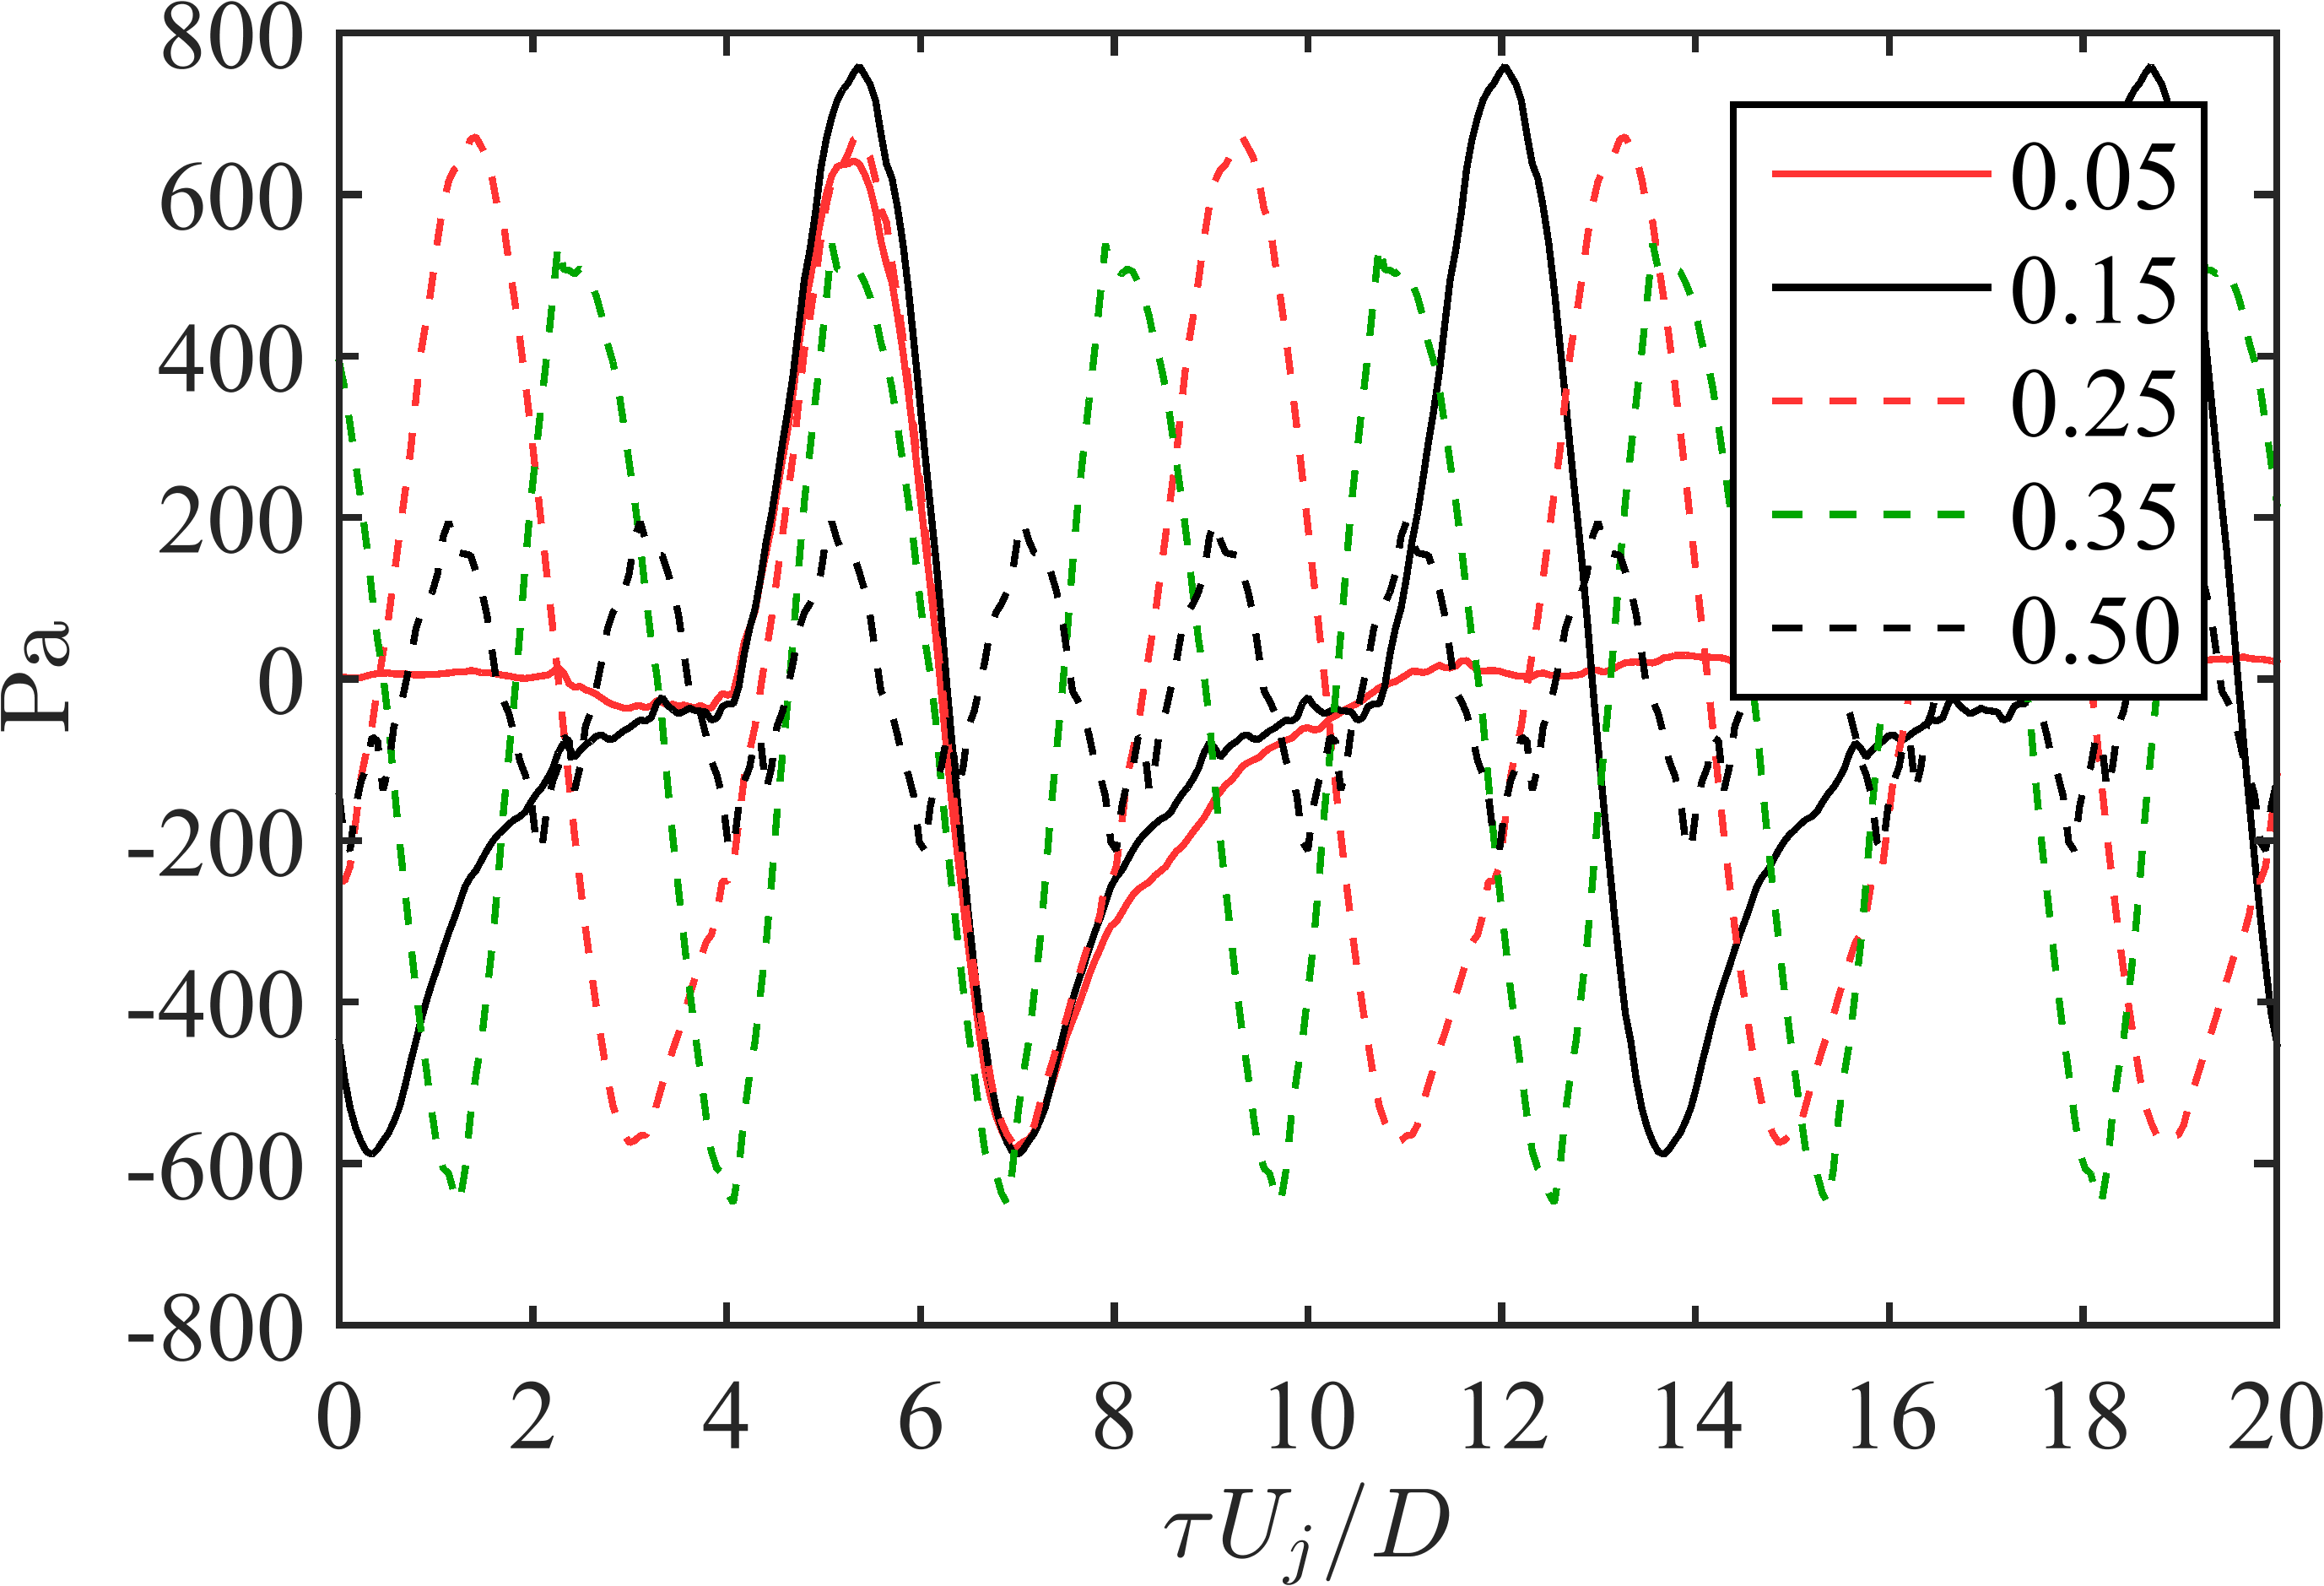
\includegraphics[width=0.45\linewidth]{Figures/ch3_nearfield_phavg_v2.png}
%		\caption{}
%		\label{fig:ch3_nearfield_phavg}
%	\end{subfigure}%
%	\begin{subfigure}{.5\textwidth}
%		\centering
		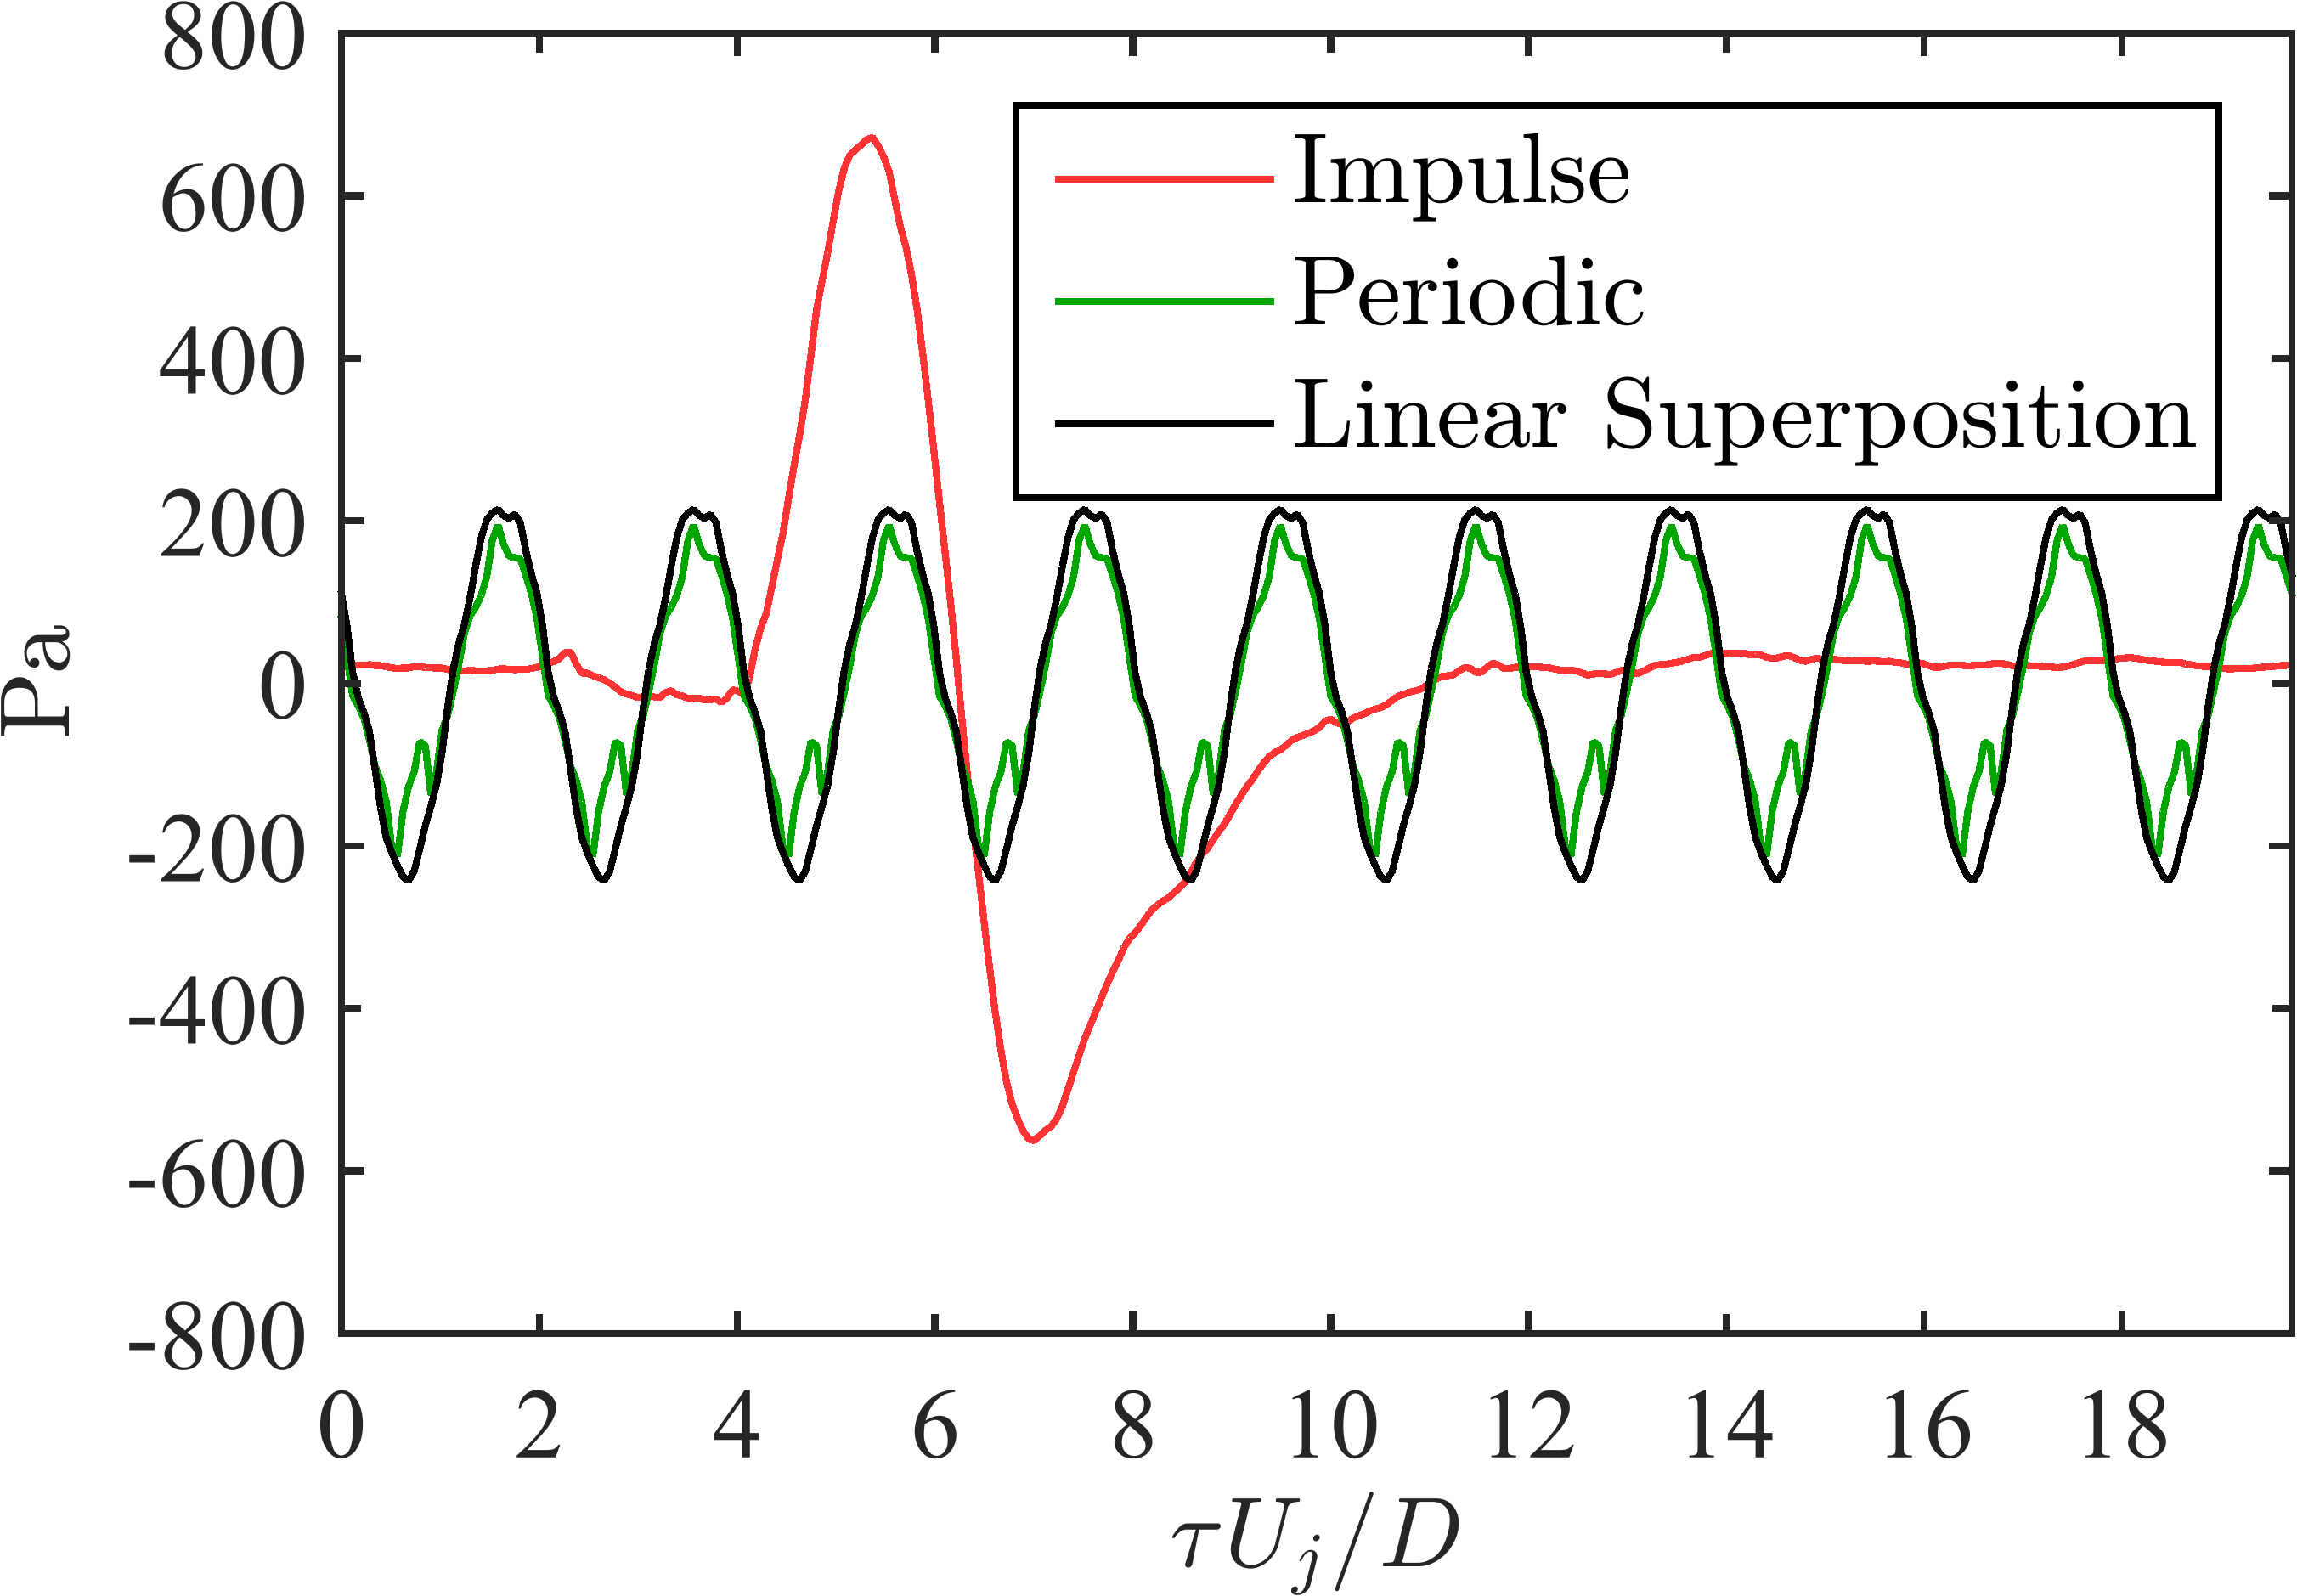
\includegraphics[width=0.45\linewidth]{Figures/ch3_nearfield_linear_v2.png}
%		\caption{}
%		\label{fig:ch3_nearfield_linear}
%	\end{subfigure}
	\caption{Phase-averaged waveforms along the first array position at $x/D = 3, r/D = 1.35$ (a) and a linear superposition of the phase-averaged waveform for the impulse excitation ($St_{DF} = 0.05$) compared against periodic excitation ($St_{DF} = 0.50$) (b).}
	\label{fig:ch3_nearfield}
\end{figure}

For a certain range of excitation frequencies ($St_{DF} \leq 0.50$ at $x/D = 2$, for example), the structures interact in a quasi-linear manner, insofar as their near-field pressure signatures are concerned. 
To be precise, the response of the jet in the irrotational near-field could be well-predicted by a linear summation of the impulse response of the jet, repeated at the periodic excitation frequency. 
This concept has been illustrated in \fig{fig:ch3_nearfield}b, where the periodic response of the jet to excitation with $St_{DF} = 0.50$ has been reproduced at $x/D = 3$. 
Additionally, a linear superposition of the impulse response for $St_{DF} = 0.05$, repeated to match the excitation frequency of $St_{DF} = 0.50$, has been overlaid. 
The linear superposition has been arbitrarily shifted in time in order to match the phase of the periodic response; this phase difference is likely due to the dependence of convection velocities on structure frequency \citep{Veltin2011} (or more accurately, structure size). 
For reference, the impulse response has also been included in the plots. 
Upstream of the end of the potential core ($x/D \simeq 6$, as will be found in \sect{sect:velocity}), the quasi-linear interaction model produces close predictions of the waveform amplitude and shape, despite the significant difference in both peak amplitude and waveform shape between the impulse and periodic responses. 

This quasi-linear interaction of the jet response to excitation is not limited exclusively to the hydrodynamically-dominated regions of the jet, but in fact holds for the acoustic far-field as well, at aft angles (where the acoustic signal is strongest and is known to correlate well with large-scale structures). 
This can be observed in \fig{fig:ch3_farfield}a, where the phase-averaged response of the jet has been plotted for the far-field signal at a polar angle of $30^\circ$. 
For legibility, only a select number of excitation Strouhal numbers have been included. 
As with the irrotational near field, the acoustic far field exhibits a compact waveform for the lowest excitation Strouhal numbers. 
Though nearly a direct inverse from the waveform observed in the hydrodynamically-dominated near field, the far-field waveform is quite reminiscent of the phase-averaged waveforms observed by \citet{Kambe1983} for the acoustic radiation towards aft angles produced by the head-on collision of vortex rings. 
At higher $St_{DF}$, a continuous oscillation between sharp expansion and compression waves is again observed, though the amplitude begins to decay above moderate excitation Strouhal numbers. 
\begin{figure}
	\centering
%	\begin{subfigure}{.5\textwidth}
%		\centering
		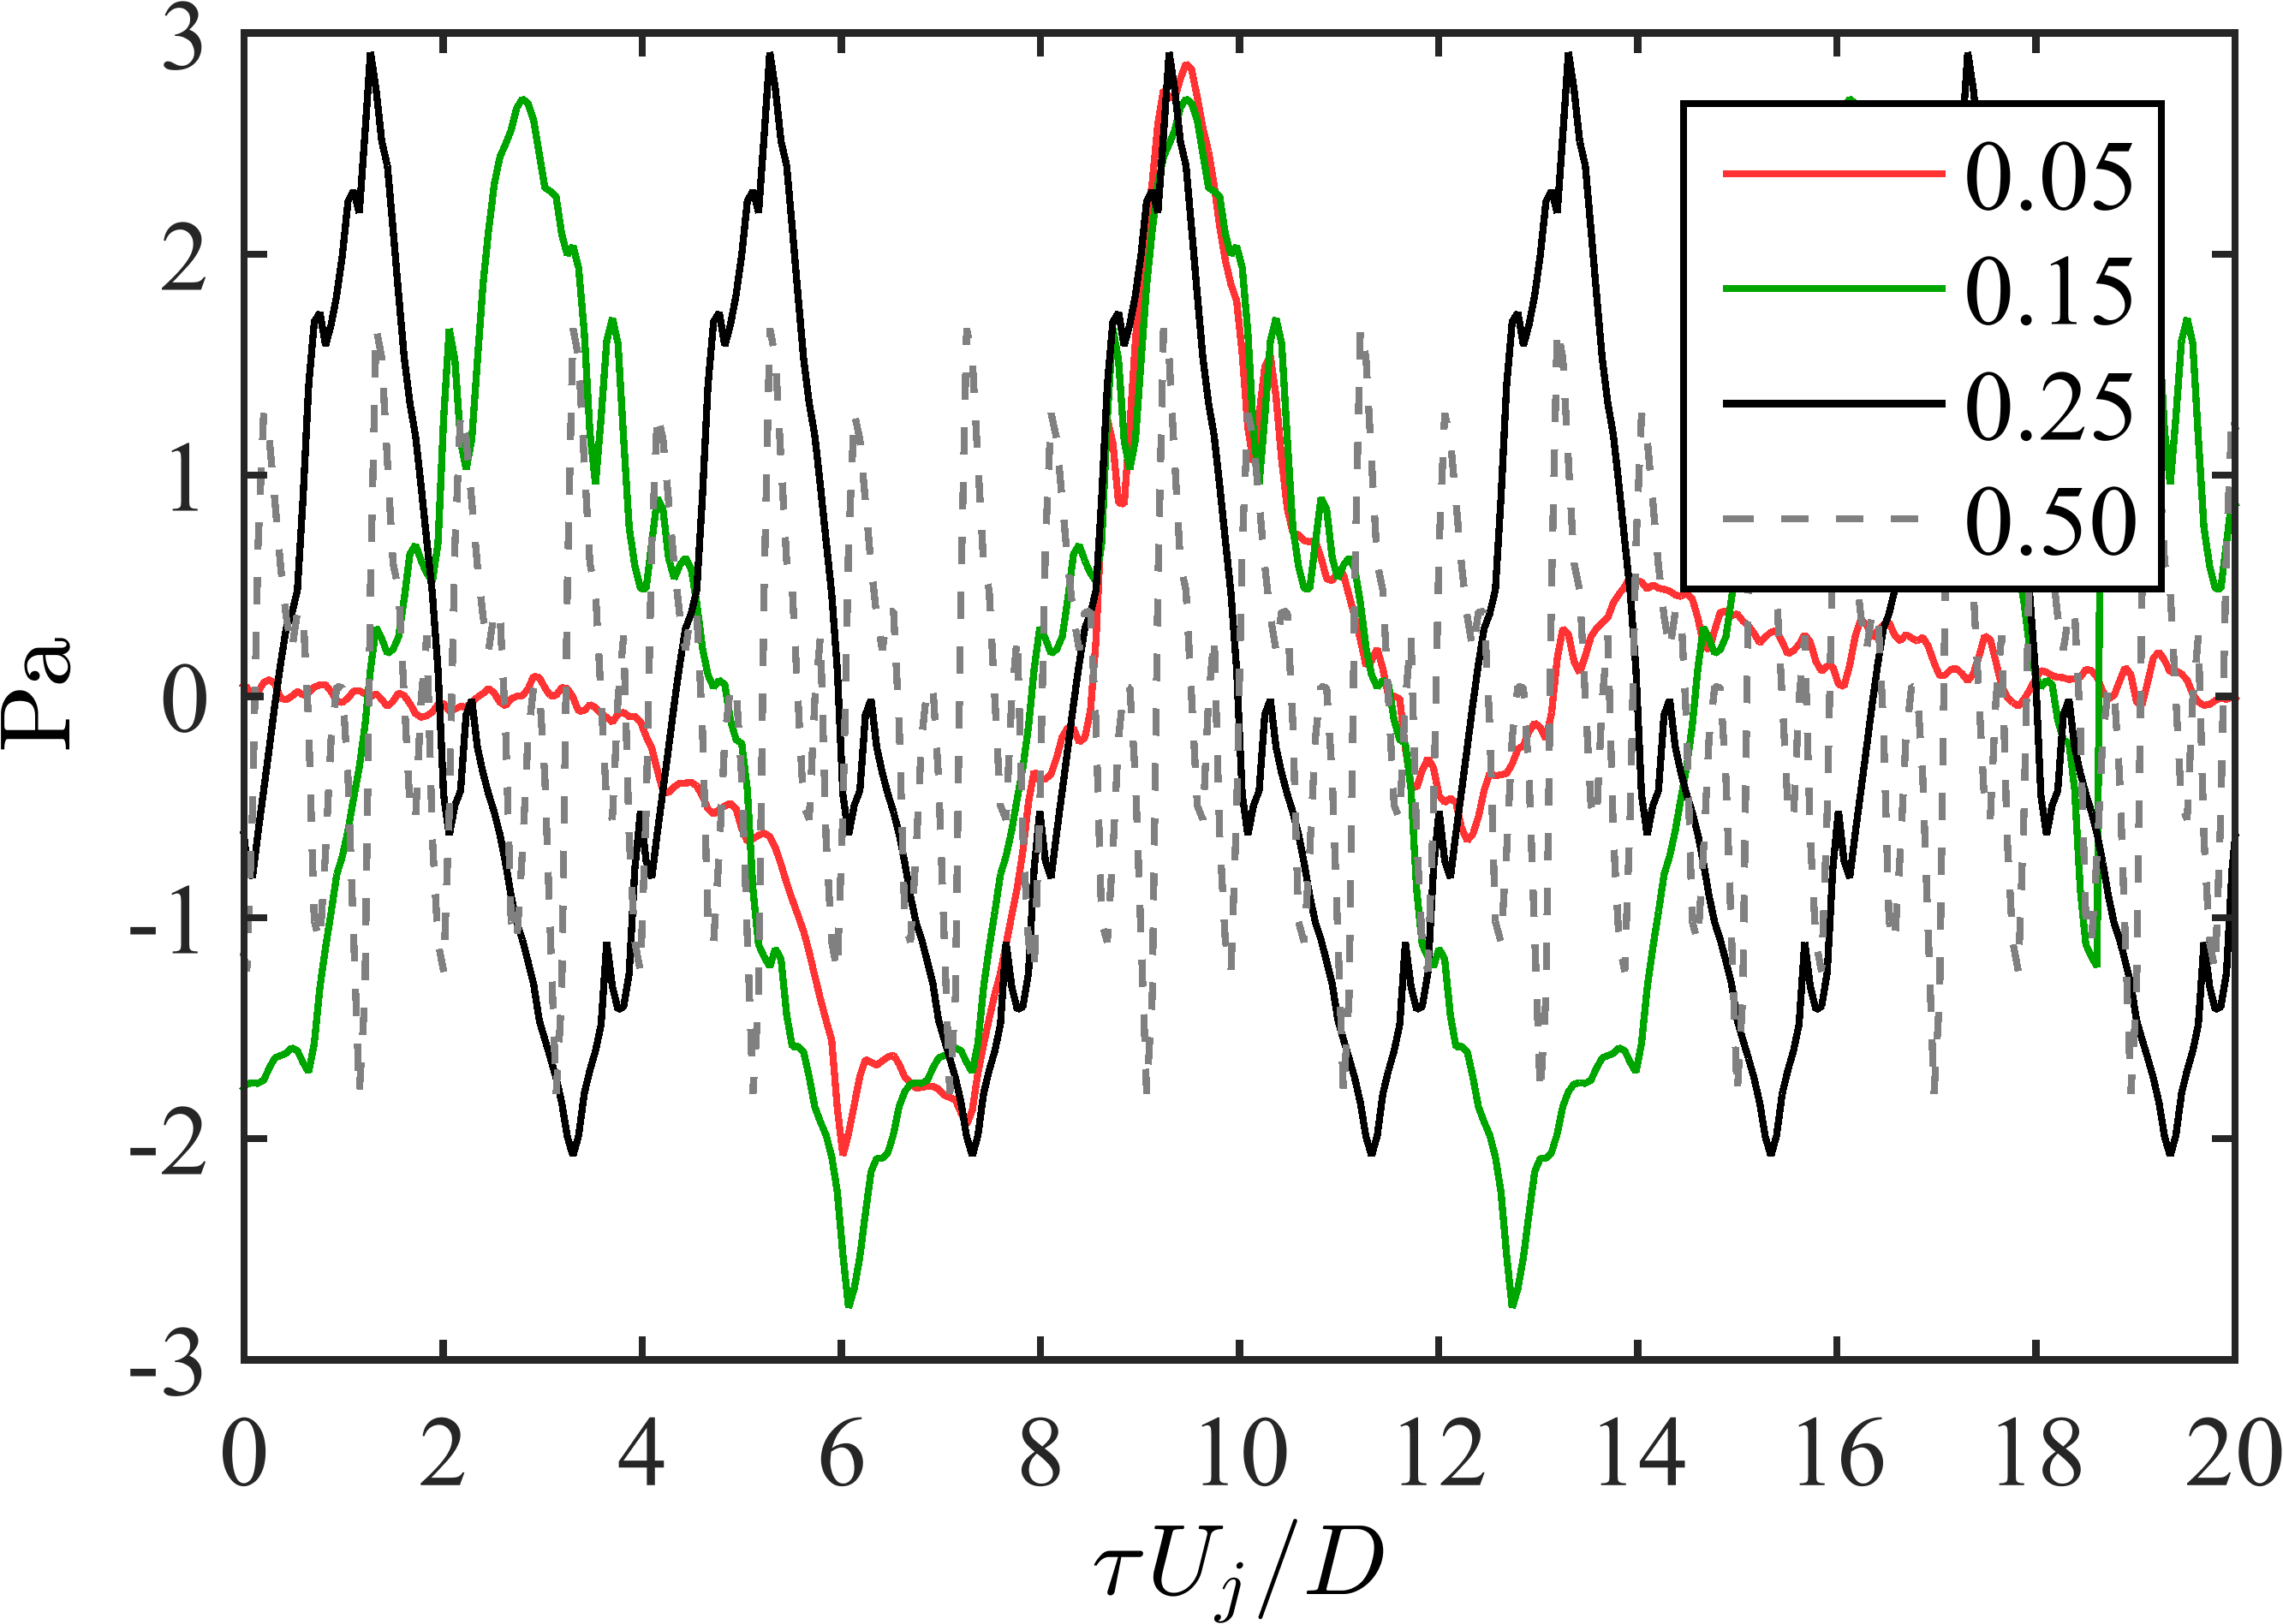
\includegraphics[width=0.45\linewidth]{Figures/ch3_farfield_phavg_v2.png}
%		\caption{}
%		\label{fig:ch3_farfield_phavg}
%	\end{subfigure}%
%	\begin{subfigure}{.5\textwidth}
%		\centering
		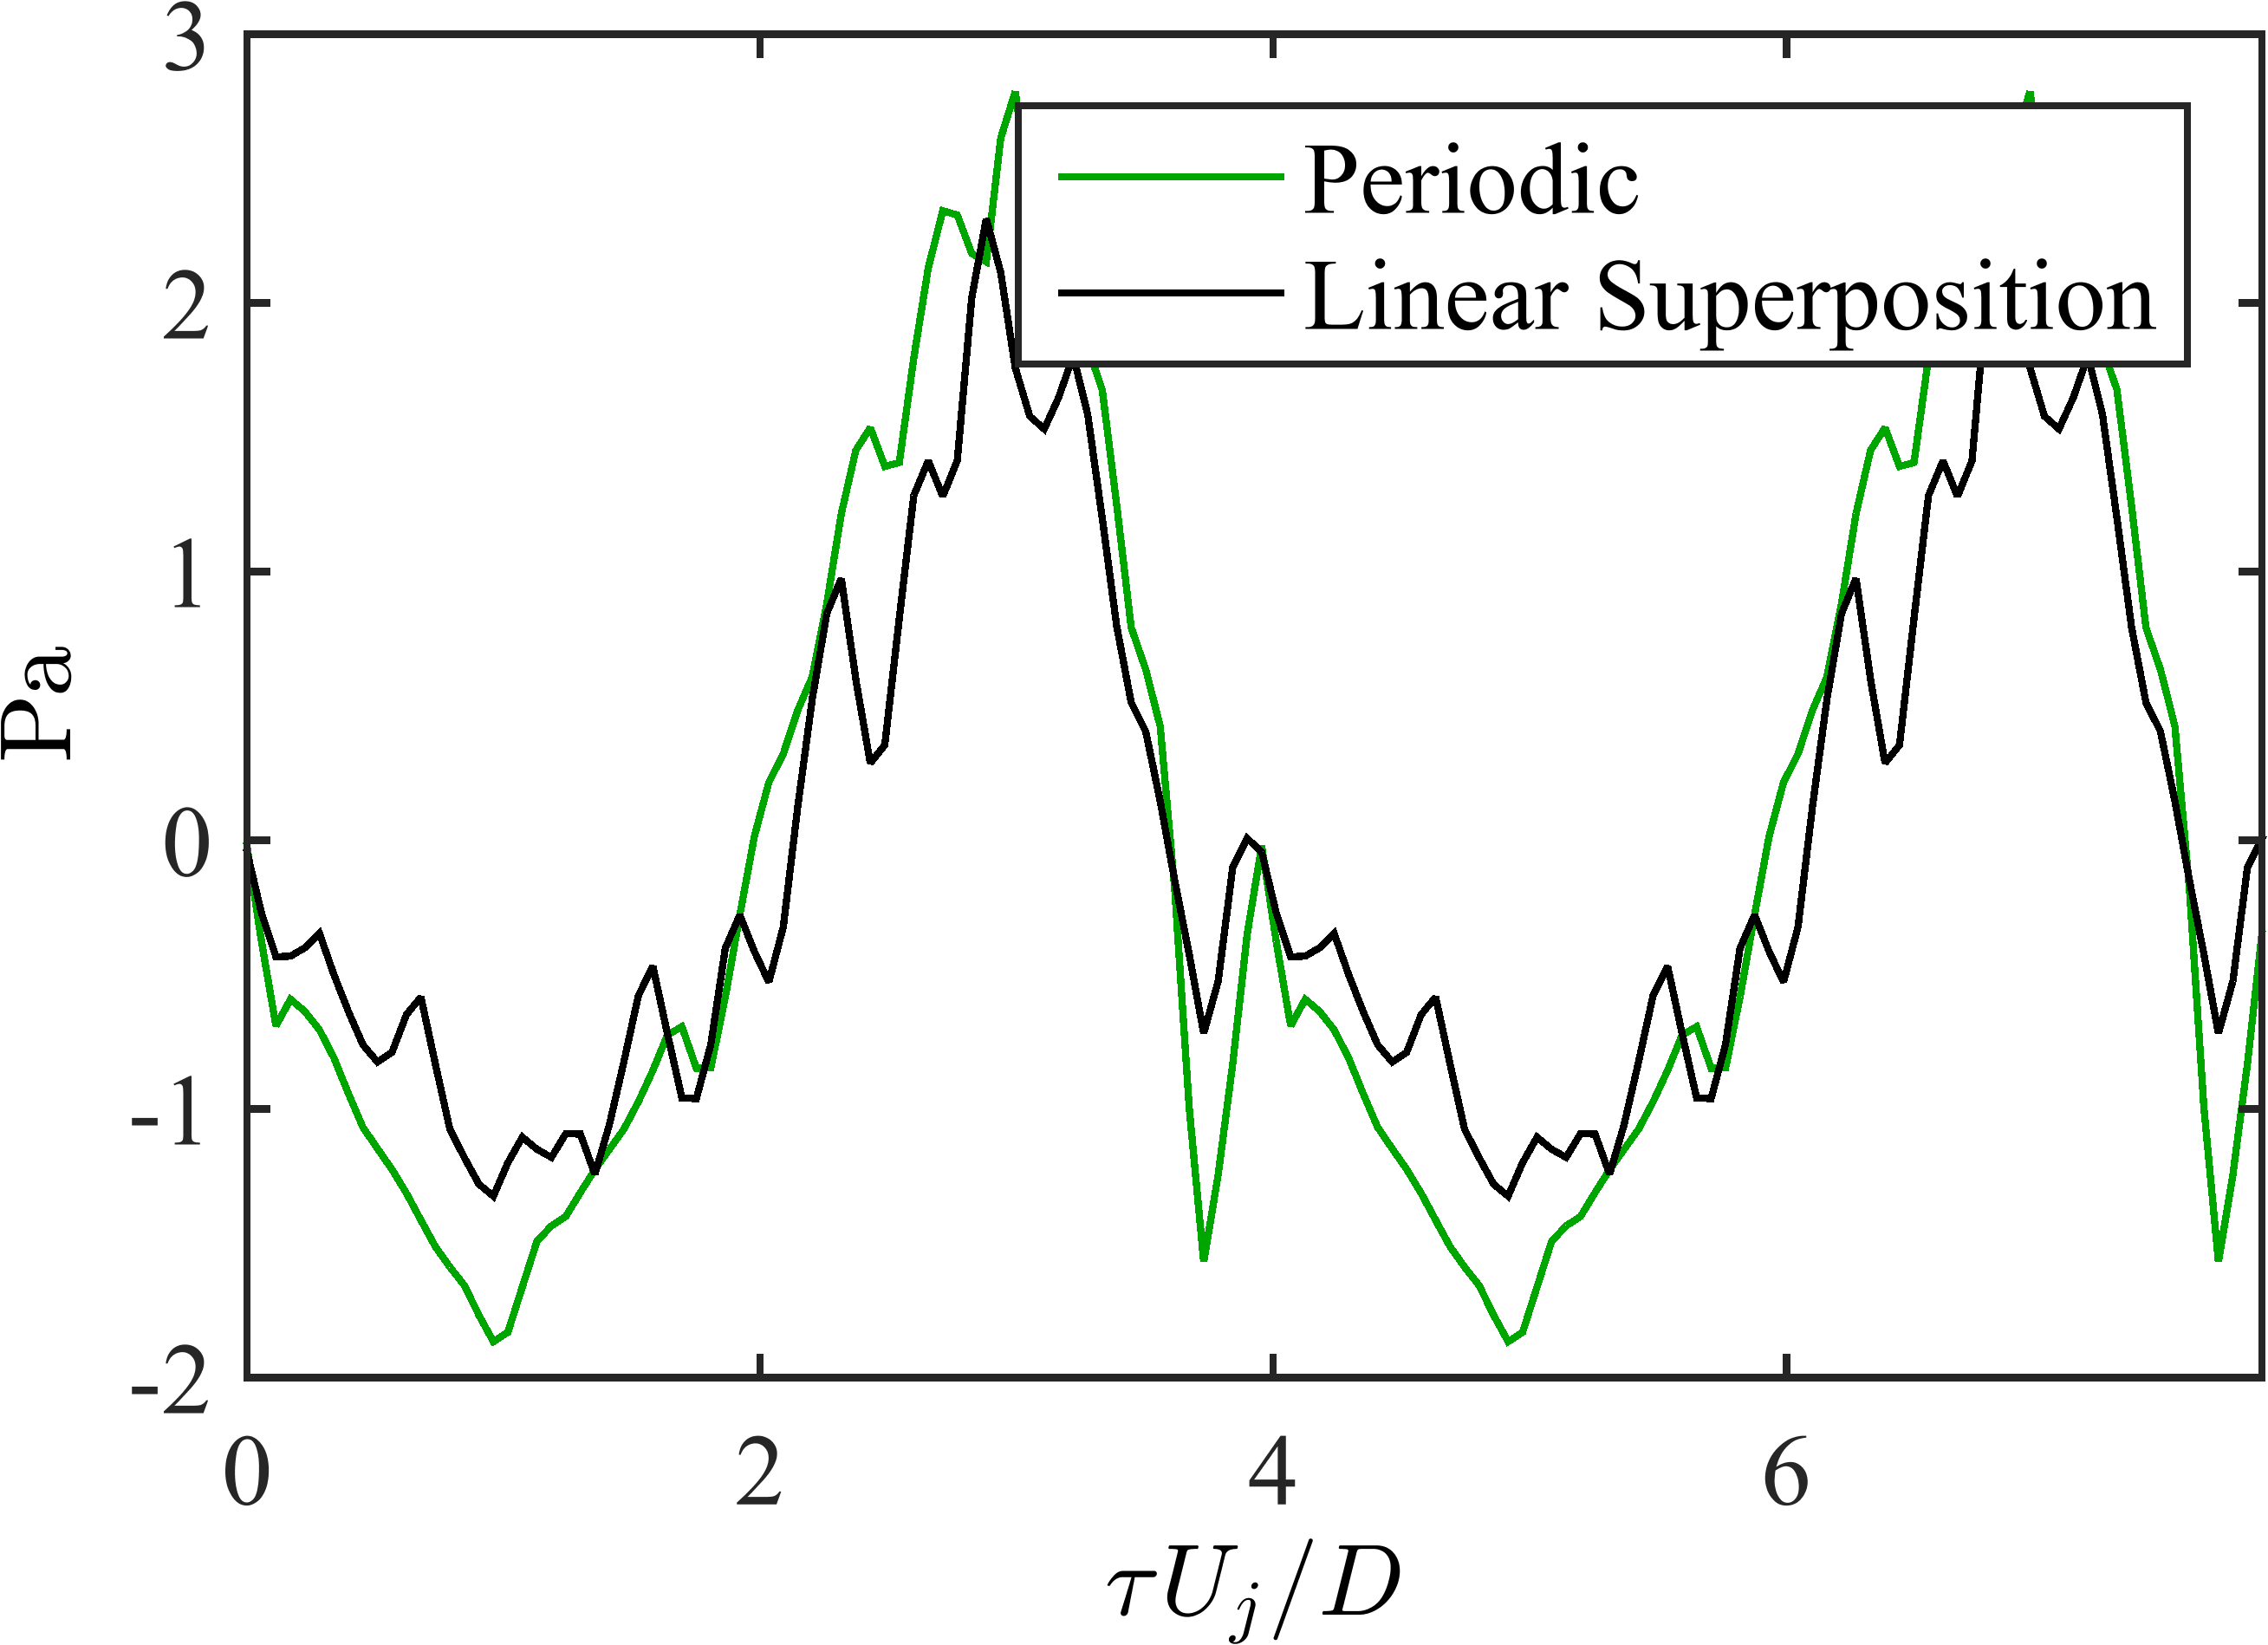
\includegraphics[width=0.45\linewidth]{Figures/ch3_farfield_linear_v2.png}
%		\caption{}
%		\label{fig:ch3_farfield_linear}
%	\end{subfigure}
	\caption{Phase-averaged waveforms of the far-field at $30^\circ$ (a) and a linear superposition of the phase-averaged waveform for the impulse excitation ($St_{DF} = 0.05$) compared against periodic excitation ($St_{DF} = 0.25$) (b).}
	\label{fig:ch3_farfield}
\end{figure}

As before, a linear superposition of the impulse response can well predict the waveform shape and amplitude at the higher excitation frequencies (\fig{fig:ch3_farfield}b), though in this case only up to $St_{DF}  = 0.25$. 
From the phase-averaged waveforms alone it is not clear whether this breakdown in the linear superposition model at the highest excitation frequencies is due to nonlinear behavior or uncertainty in the phase-averaging. 
Results comparing the linear superposition of the impulse response against the measured periodic response at $St_{DF}  = 0.35$ are shown in \fig{fig:ch3_farfield_nonlinear}.
Some similarities may be found in the waveform shape and amplitude, but overall it is clear that the acoustic response of the jet to excitation at $St_{DF}  = 0.35$ is substantially modified from the response at lower frequencies.
Though this is hardly conclusive in its own right, this result does suggest either changing or competing acoustic source mechanisms are present in these excited jets.
The phase-averaged waveforms were also investigated at polar angles of $60^\circ$ and $90^\circ$; however a clear waveform was not identifiable over the statistical uncertainty inherent in the phase-averaging process (likely due to the superdirective character of the acoustic radiation \citep{Crighton1990}, which renders the amplitude at sideline angles too low to be detectable).
Additional details and analysis of the phase-averaged near- and far-field signals can be found in \citet{Crawley2015}.
\begin{figure}
	\centering
	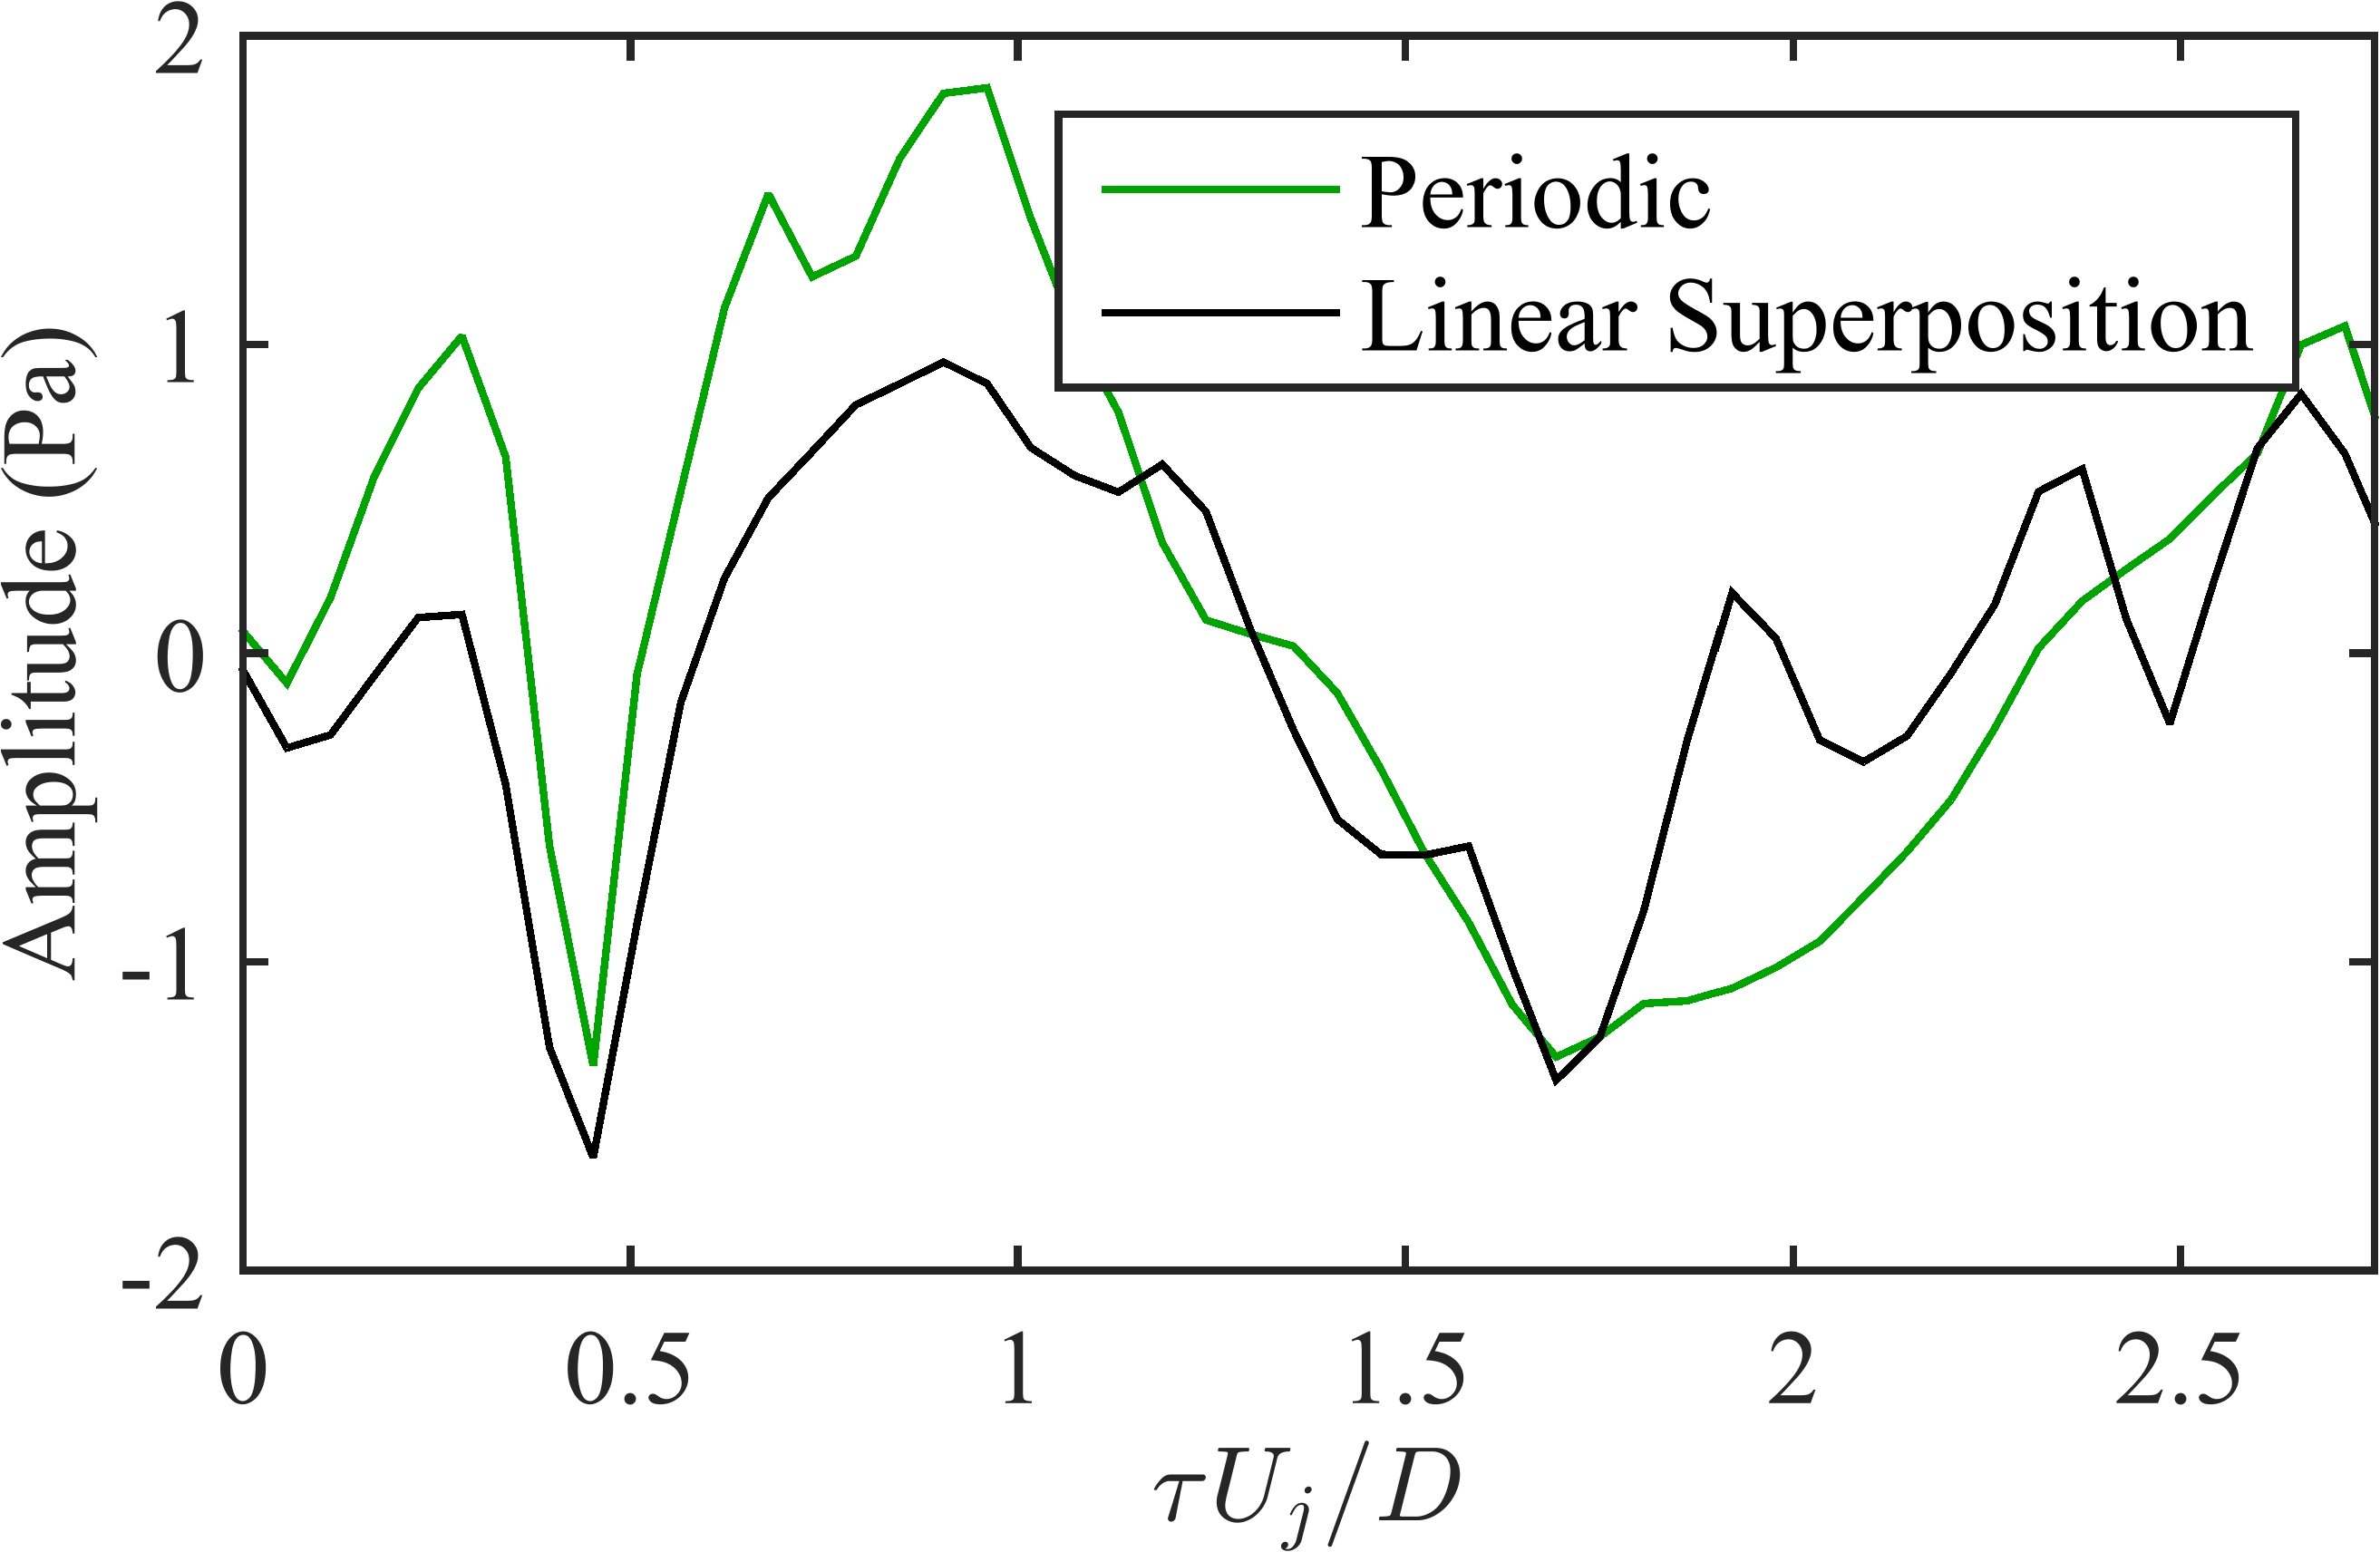
\includegraphics[width=0.45\linewidth]{Figures/ch3_farfield_linearsuperposition_st035_v2.png}
	\caption{Linear superposition of the phase-averaged impulse response to excitation against the measured periodic response for $St_{DF} = 0.35$ at the  $30^\circ$ far-field microphone.}
	\label{fig:ch3_farfield_nonlinear}
\end{figure}

\subsection{Excited versus Natural Structures}
The effect of excitation on the turbulent jet is to generate highly energetic coherent structures which persist downstream for several lengthscales.
As can be seen by the strong tonal energies observed for the excited jets in figure \fig{fig:sect_nearfield_spectra_prms}a, the near-field response to these structures contains energy at the fundamental excitation frequency and numerous higher harmonics.
As the excitation frequency increases from the impulse-excitation regime to the periodic, the dominance of the fundamental tone over the higher harmonics becomes more pronounced, though this is an artifact of the Fourier transform and not a fundamental physical phenomenon. 
The presence of these highly-energetic structures can also lead to an amplification of the broadband turbulence, over a wide band of frequencies both above and below the fundamental excitation frequency.
It also produces a continuous upstream shift in the root-mean-squared peak amplitude of the phase-averaged, as can be seen in \fig{fig:sect_nearfield_spectra_prms}b, with the maximum being obtained near $St_{DF} \simeq 0.3$ (which is commonly identified as the jet column instability frequency in natural jets).
However, the fluctuation intensities as a function of frequency in the excited jets saturate much further upstream than in the natural jet ($x/D \simeq 3$ for $St_{DF} \simeq 0.3$ rather than downstream near the end of the potential core at $x/D \simeq 6$).
In light of this issue, an investigation of the coherent structures in the natural jet and their comparison against the excited was deemed pertinent to the analysis of the excited structure dynamics.
\begin{figure}
	\centering
	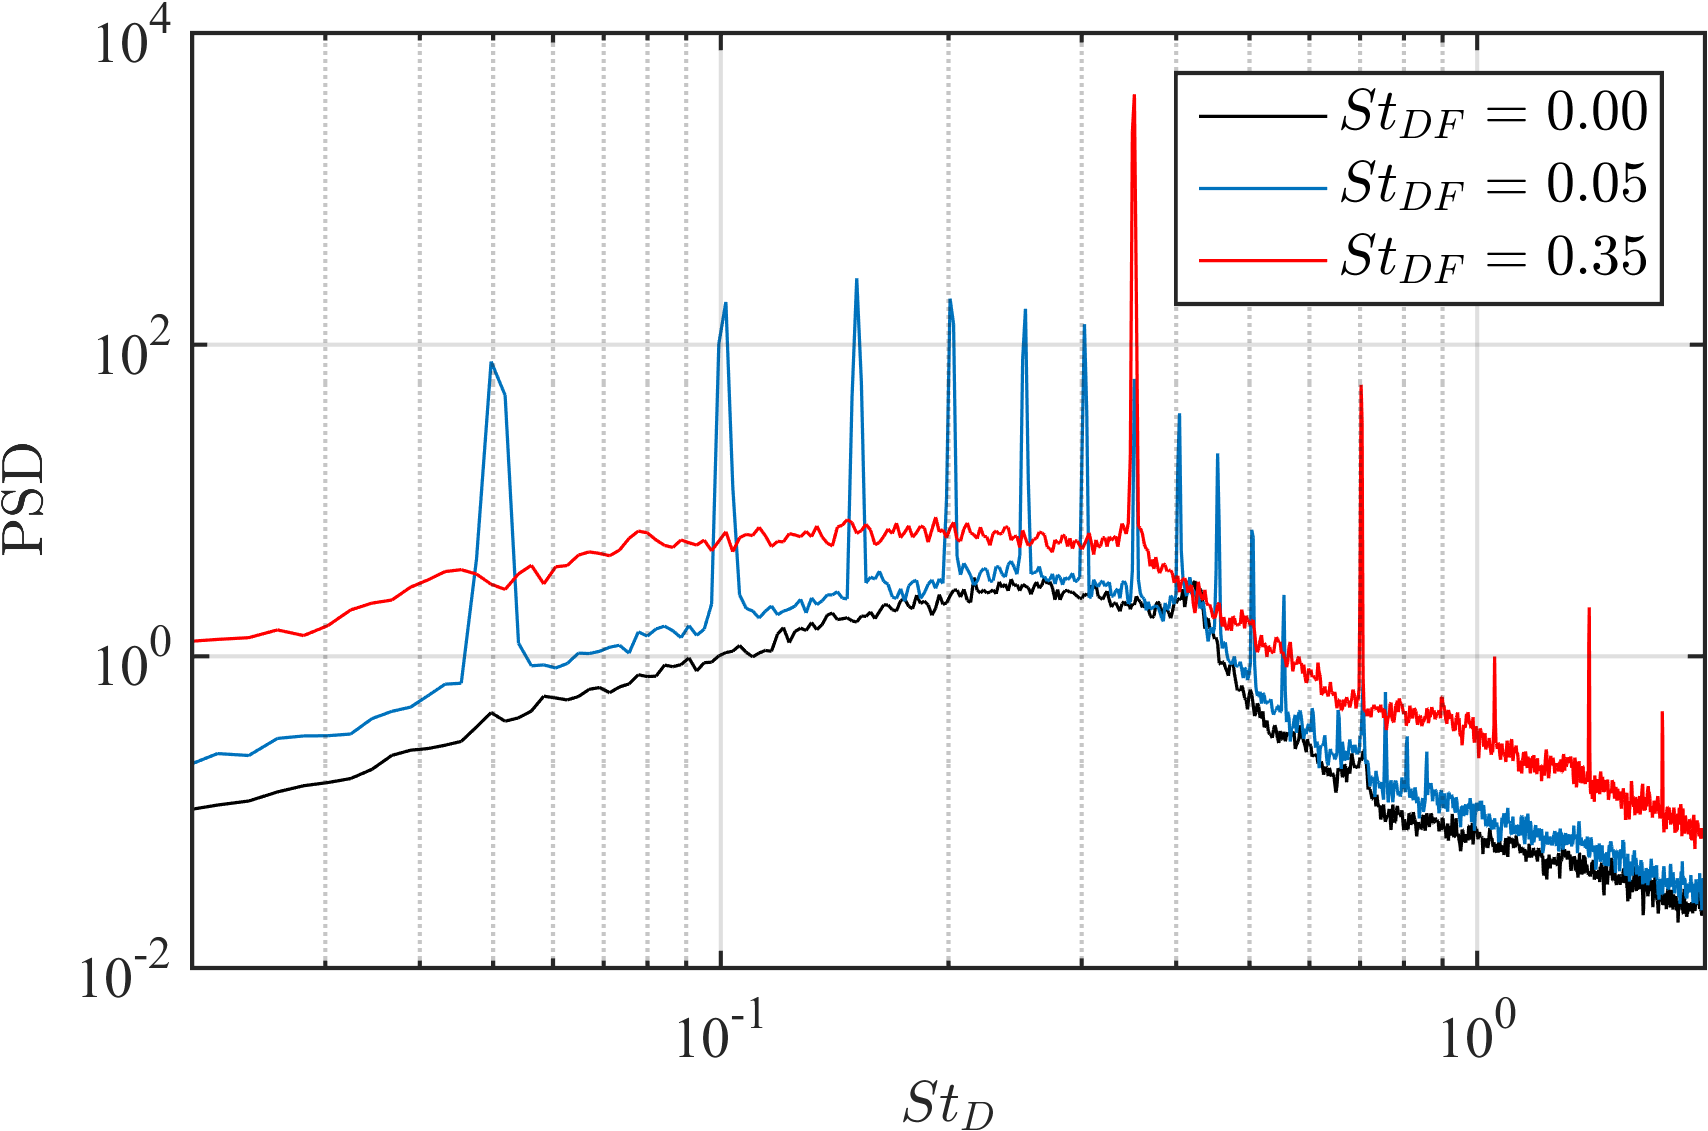
\includegraphics[width=0.44\linewidth]{Figures/sect_nearfield_spectra.png}
	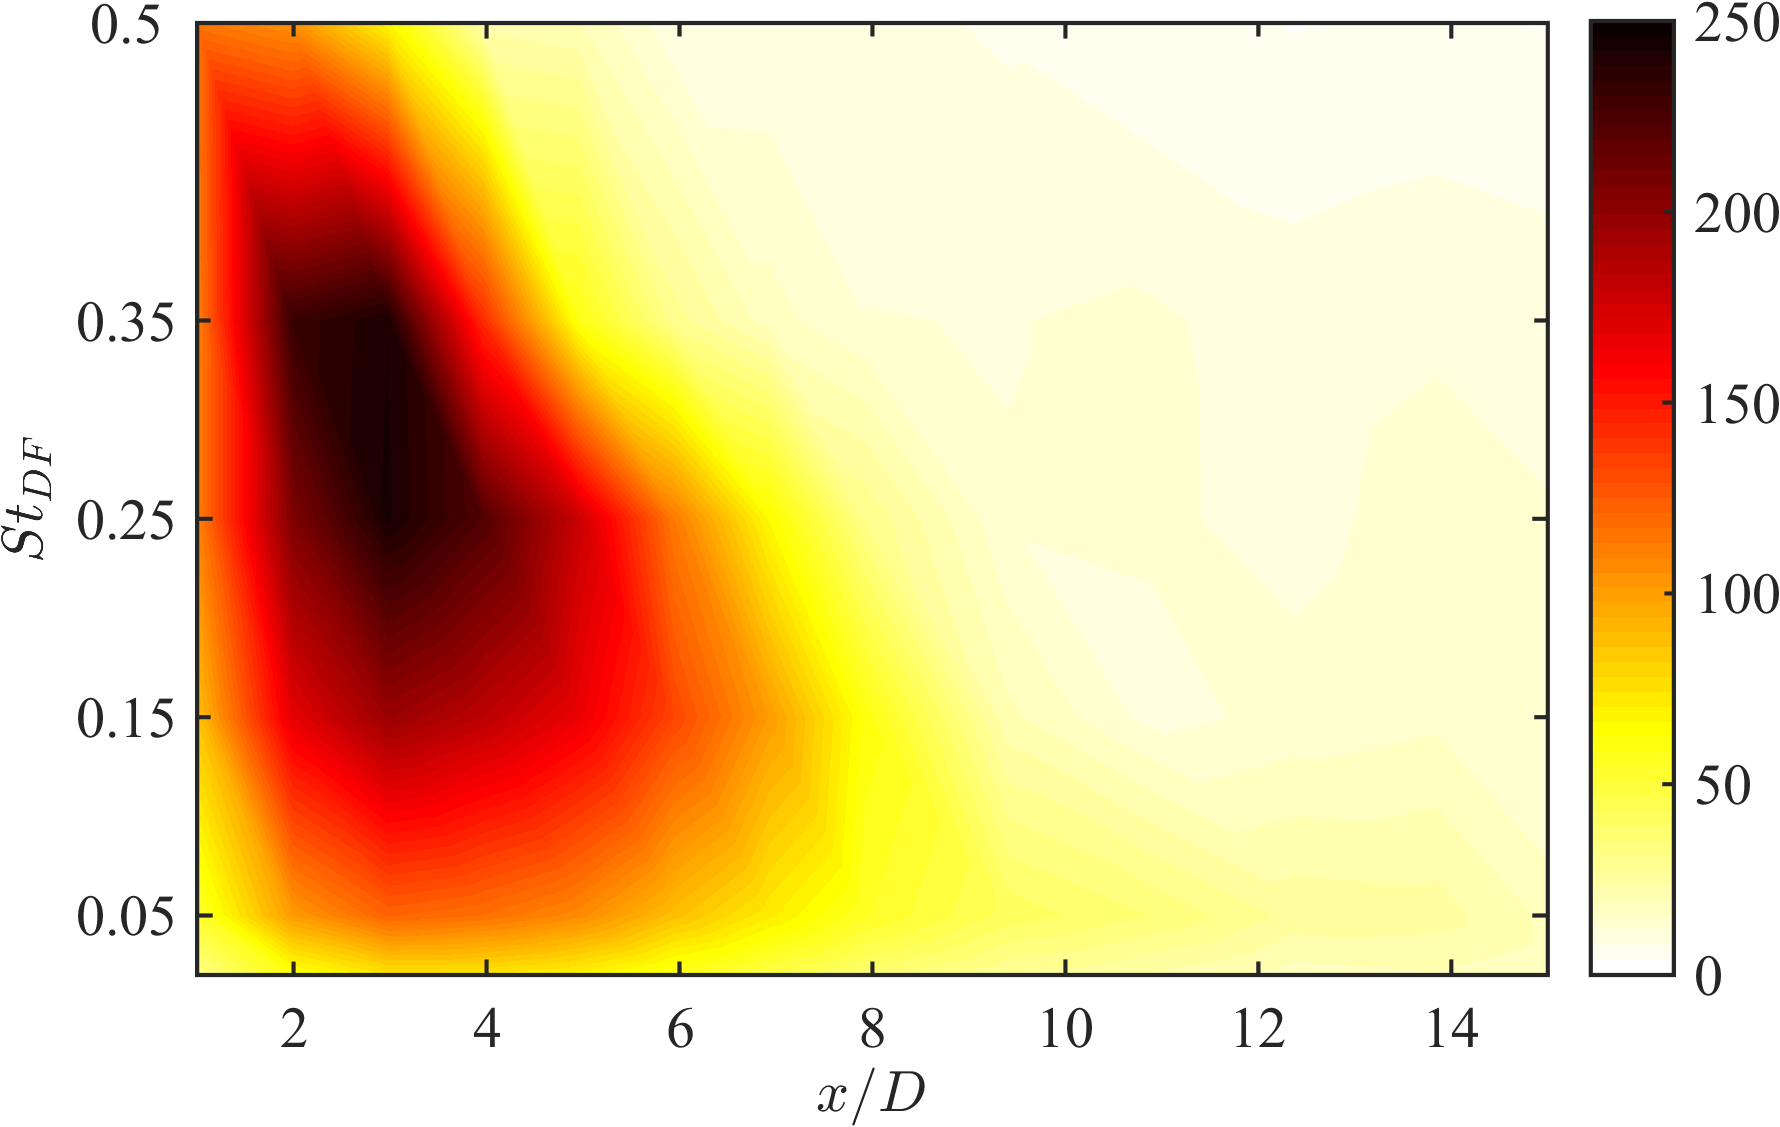
\includegraphics[width=0.46\linewidth]{Figures/sect_nearfield_prms.png}
	\caption{Power spectral densities of the raw near-field pressure at $x/D = 3$ (a) and root-mean-squared pressure fluctuations of near-field pressure at (b).}
	\label{fig:sect_nearfield_spectra_prms}
\end{figure}

Obviously, it is not possible to use standard phase--averaging with the unforced case since the natural turbulent structures, although dominated by Strouhal numbers related to the instabilities in the jet, contain a broad range of energetic scales with no fixed phase relationship. 
It is necessary then to use an alternative averaging method in order to extract a coherent signature of the unforced jet turbulent--structures.
Instead of phase-averaging a conditional--averaging method, specifically wavelet--conditioning, was applied to the unforced and forced cases to determine how closely the forced structures relate to the natural structures in the jet.
A wavelet decomposition was chosen as it affords an efficient methodology for analyzing intermittent events in a given signal due to the finite energy of its basis functions.
This is in contrast to the more standard Fourier decomposition in which continuously-oscillating basis functions spread information from a single instance in time across all transform coefficients.
For this reason, the use of the wavelet decomposition has become increasingly common in aeroacoustic research; an overview of the wavelet transform and its applications to turbulence and acoustics can be found in \citet{Farge1992}.
The wavelet decomposition is expressed as follow:
\begin{equation}\label{eqn:waveletDecomposition}
\tilde{w} \left( s, \tau \right) = \frac{1}{\sqrt{ \left| s \right|}} \int_{-\infty}^{+\infty} p \left( t \right) \overline{\Psi}\left( \frac{t - \tau}{s}\right) dt,
\end{equation}
where $s$ is the wavelet scale, which is inversely proportional to Fourier frequency, $\tau$ is the time--shift as in the Short Time Fourier Transform (STFT) formulation, $\overline{\Psi}$ is the complex conjugate of the so--called mother wavelet. The wavelet decomposition is as the STFT, a convolution of the signal to analyse with a family of functions, here the wavelets family. To get this wavelet family, which is also called the wavelet daughters, the mother wavelet is stretched/compressed and shifted. The strength of the wavelet decomposition with regards to STFT is the variation of the time--scale, which for STFT would correspond to its window. This allows a more localized information. In STFT the size of the window is fixed and the frequency is changing in order to retrieve the frequency content of the analysed signal while in the wavelet decomposition it is the time--scale (size of the window) which is different and the frequency is fixed. This difference allows to the wavelet decomposition to be more flexible and have a better resolution at both high and low frequencies.

Wavelet--based conditional averaging has been used previously for structure identification in jets and other turbulent flows \citep{Camussi1997,Camussi1999,Guj1999,Camussi2002,Guj2003}.
The technique is based on the Local Intermittency Measure (LIM) \citep{Farge1992}:
\begin{equation}
\label{eqn:LIM}
L(s, \tau) = \frac{\tilde{w}^{2}(s, \tau)}{\left<\tilde{w}^{2} (s, \tau)\right>_{\tau}},
\end{equation}
where $w^{2}(s, \tau)$ is the local energy for a specific time and scale, and $\left< \bullet \right>_{t}$ represents a time average. Simply put, the LIM is the ratio between the local energy of the wavelet coefficient for a specific time and scale $(\tau, s)$ and a time-averaged energy at the same scale $s$. The LIM was demonstrated to be a well-suited indicator for coherent structure identification \citep{Camussi1997}.  The LIM provides information about the instantaneous fluctuation of energy and by choosing a proper threshold $T$ it is possible to select a set of times $\{\tau_{i}\}$ corresponding to intermittent, energetic events in a signal.

Several methods exist in order to select the threshold: using an arbitrary threshold, an iterative process to retrieve as specific value of the Flatness Factor (skewness, forth moment), or by evaluating the Merit index \citep{Grassucci2015}. 
In the present study, a new method inspired by the merit coefficient was used to select a proper threshold. 
In contrast to the merit coefficient method, which uses a global threshold across all scales, the new method iterates at each scale to identify the proper threshold per \eq{eqn:tEvaluation}

\begin{equation} \label{eqn:tEvaluation}
R(T) = -\frac{\log\left(\frac{N_p}{N_m}\right)}{\log\left(\frac{\sigma_{w_p}}{\sigma_{w_m}}\right)}.
\end{equation} 
% \begin{enumerate}
% 	\item Select a first threshold to initiate the iterative process (1 in the present case)
% 	\item Evaluate the coefficient
% 	\begin{equation}
% 	R(T) = -\frac{\log\left(\frac{N_p}{N_m}\right)}{\log\left(\frac{\sigma_{w_p}}{\sigma_{w_m}}\right)}
% 	\end{equation}
% 	\item Re-evaluate $T$
% 	\item Iterate points 2 and 3 until $T$ achieve the maximum of $L$ for the scale under analysis
% \end{enumerate}
where $N_p$ is the length of the set $\{L > T\}$, $N_m$ is the length of the set $\{L \leqslant T\}$, $\sigma_{w_p}$ the standard deviation of the set $\{w\left( \tau_p\right) | L\left( \tau_p \right) > T\}$ and $\sigma_{w_m}$ the standard deviation of the set $\{w\left( \tau_m\right) | L\left( \tau_m \right) \leqslant T\}$.
The outcome of this iterative process is a set of vectors: one containing the different value of $T$ and the second the different value of $R(T)$. The threshold for the analysis is selected to correspond to the maximum of $R(T)$.

The next step is to get similar results to those obtained with the phase--average. In order to get the signatures, a conditional--average (\eq{eqn:ensembleAverage}) using the set of times $\{\tau_{i}\}$ is performed. In one way, the conditional--average and phase--average are similar: the set of times $\{\tau_{i}\}$ replaces the phases on which the phase--average is performed. At each time location corresponding to a peak of energy, a window $W$ of fixed time--length $l_{W}$ is selected from the original signal $p \left( t \right)$. The conditional--average, $\tilde{p}$ is calculated from this set of windows:
\begin{equation} \label{eqn:ensembleAverage}
	\tilde{p}^n_{m}\left( W \right) = \left< p_{m} | P_{k} \right>_{\tilde{\tau}^n_{s}} = \frac{1}{N^n} \sum^{N^n}_{i = 1} p_{m}\left(\xi_{i}\right),
\end{equation}
where the superscript $n$ and subscript $m$ stand for the position of the reference signal and of any other signal of the array, respectively. Also, the subscript $s$ stands for the scale, $N^n$ is the number of detected events, $\tilde{\tau}^n_{s}$ is the set of corresponding times for a specific scale $s$ at which these events are occurring and $\{\xi_{i}\}$ is the interval surrounding each peak, $\xi_{i} \in \left[ \tilde{t}_{i} - \frac{l_W}{2}, \tilde{t}_{i} + \frac{l_w}{2} \right]$, $\tilde{t}_{i} \in \tilde{\tau}^n_{s}$.
A first analysis using \eq{eqn:ensembleAverage} was performed on the microphones line--array. A second analysis was then performed by doing the conditional--average only with peaks with negative/positive value in the real domain (pressure).

\begin{figure}
	\centering
	\includegraphics[width=0.45\linewidth]{Figures/negativePeak.eps}%
	\includegraphics[width=0.45\linewidth]{Figures/positivePeak.eps}\\	
	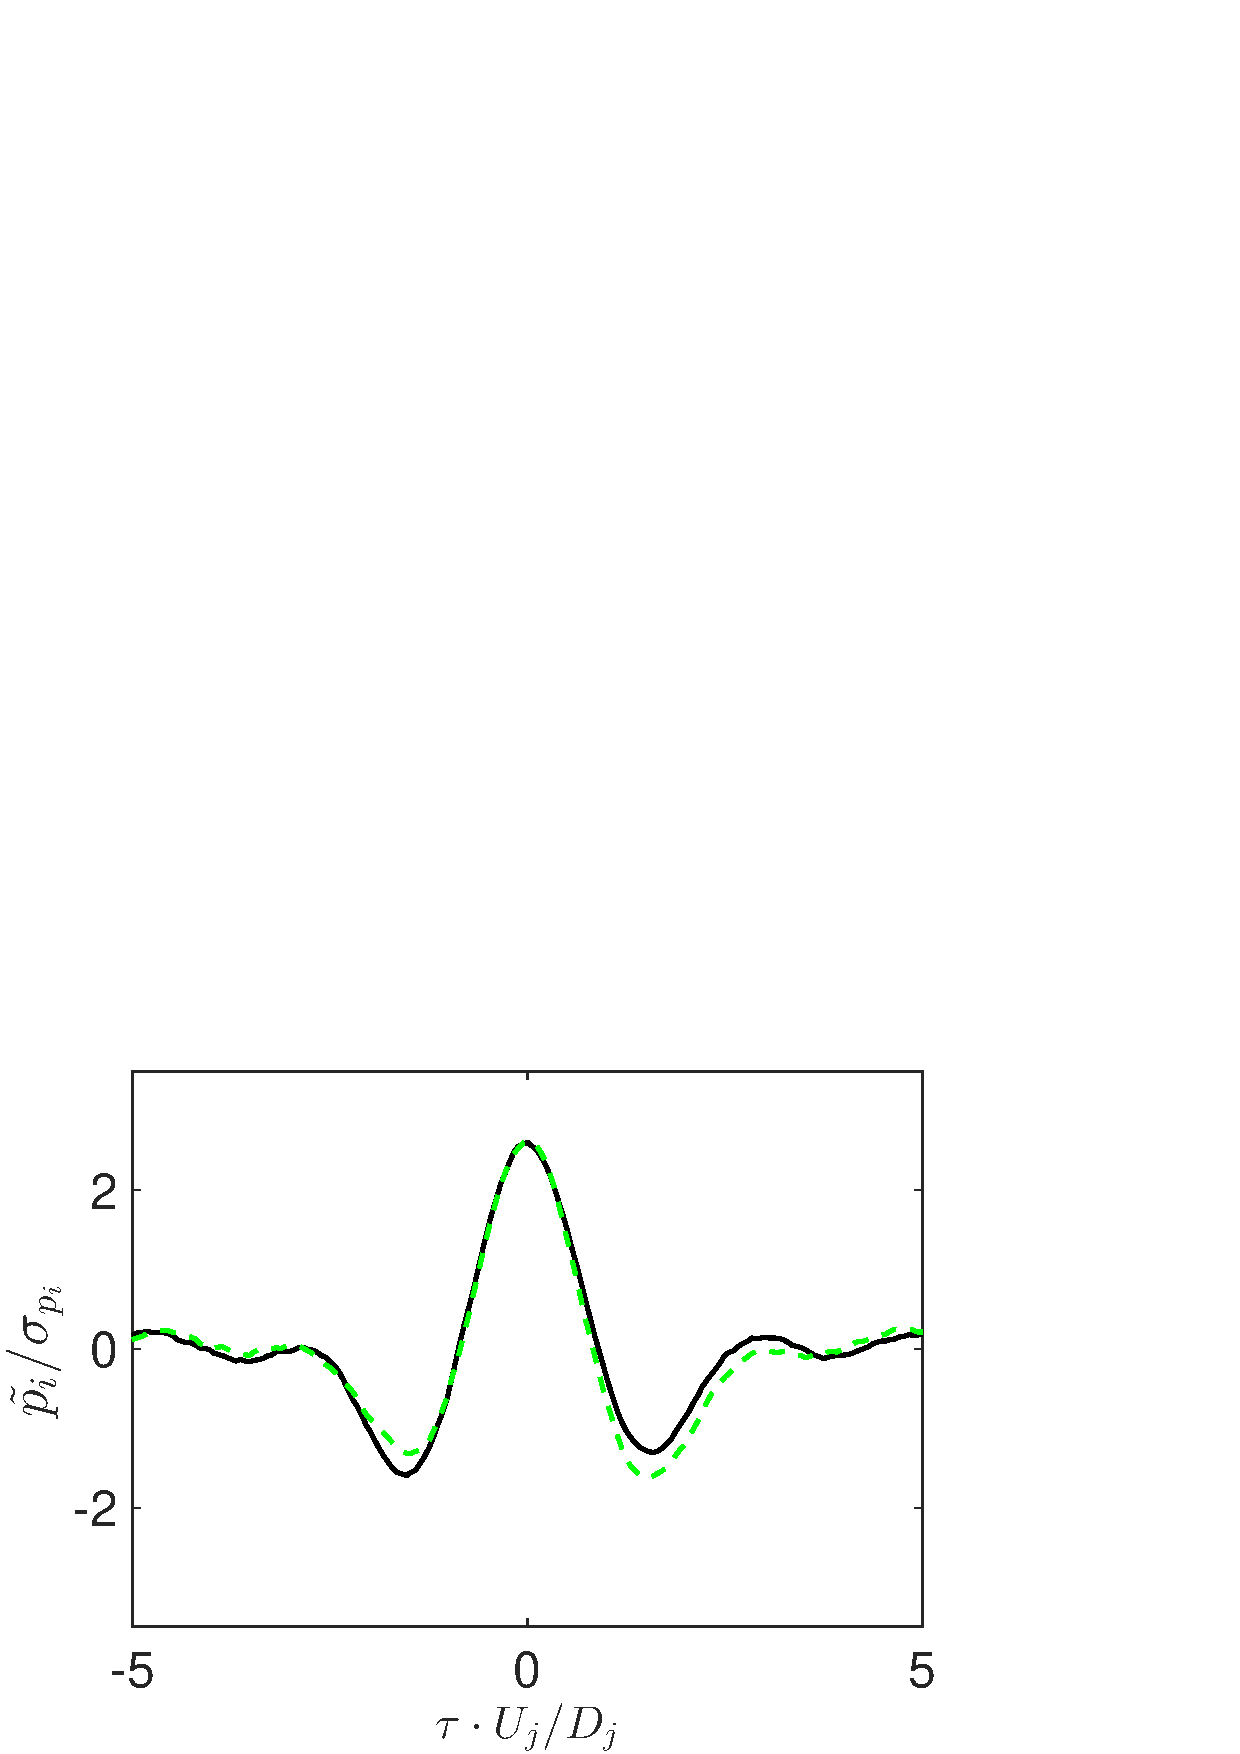
\includegraphics[width=0.45\linewidth]{Figures/compPeaks}
	\caption{Auto--conditioning signatures of the signal at $x/D = 3$} \label{fig:compPeaks}
\end{figure}
\fig{fig:compPeaks} presents the two subfigures for the different cases (negative/positive peaks) and a third subfigure to compare them.
\begin{itemize}
  \item $(a)$ conditional--average (\eq{eqn:ensembleAverage}) using only the negative peaks
  \item $(b)$ only the positive peaks
  \item a comparison between the two previous one ($(a)$ was inverted in order to compare it to $(b)$)
\end{itemize}
\fig{fig:compPeaks}c presents the resemblance between the signature of subfigures (a) and (b) on which the conditional--average was performed using only negative or positive peaks (it is important to understand that the differentiation is done by evaluating the value of each peak in the real domain and not in the LIM/wavelet domain). At this point, it is believed to be the result of the passage of two successive large scale turbulent--structures, in the zone where their interaction take place.
The formulation of the conditional--average was modified to take this observation into account and reformulated as follows:
\begin{equation} \label{eqn:condAvgSign}
\tilde{p}_{m}^n\left( W \right) = \left< p_{m} | P_{k} \right>_{\tilde{\tau}^n_{s}} = \frac{1}{N^n} \sum^{N^n}_{i = 1} sign\left( p_{n} \left( \tilde{t}_{i} \right) \right) p_{m} \left( \xi_{i} \right),
\end{equation}
$sign\left( p_{n} \left( \tilde{t}_{i} \right) \right)$ is introduced to take into account the sign of the peak in the real domain. This operation might be unnecessary for an experimental database (with a long time--series) but for a numerical database which is strongly limited in its time duration it improves the results obtained with the wavelet--conditioning.
The conditional--average using \eq{eqn:ensembleAverage} with all the peaks present (not presented here) is not relevant as additional proof for the separation between negative/positive peaks.
When the conditional--average is performed on a signal $p_{n}$ by using its own set of times ${\tilde{\tau}^n_{s}}$, making $n = m$; it becomes the auto--conditioning. If the conditional--average of a signal $p_{m}$ is done by using the set of times of a signal $p_{n}$, and so $n \neq m$; it is then called the cross--conditioning. The auto/cross--conditioning are presented in \fig{fig:condNcond}: the top is the auto--conditioning where the selection of $W$ is done in the reference signal $n$; and the bottom is the cross--conditioning of another signal $m$ where $W$ is centered around the times obtained with signal $n$. For more information about the wavelet--transform, see \cite{Farge1992}. The cross--conditioning is only presented in theory but no results with valuable meaning were obtained for this specific study.
\begin{figure}
	\centering
	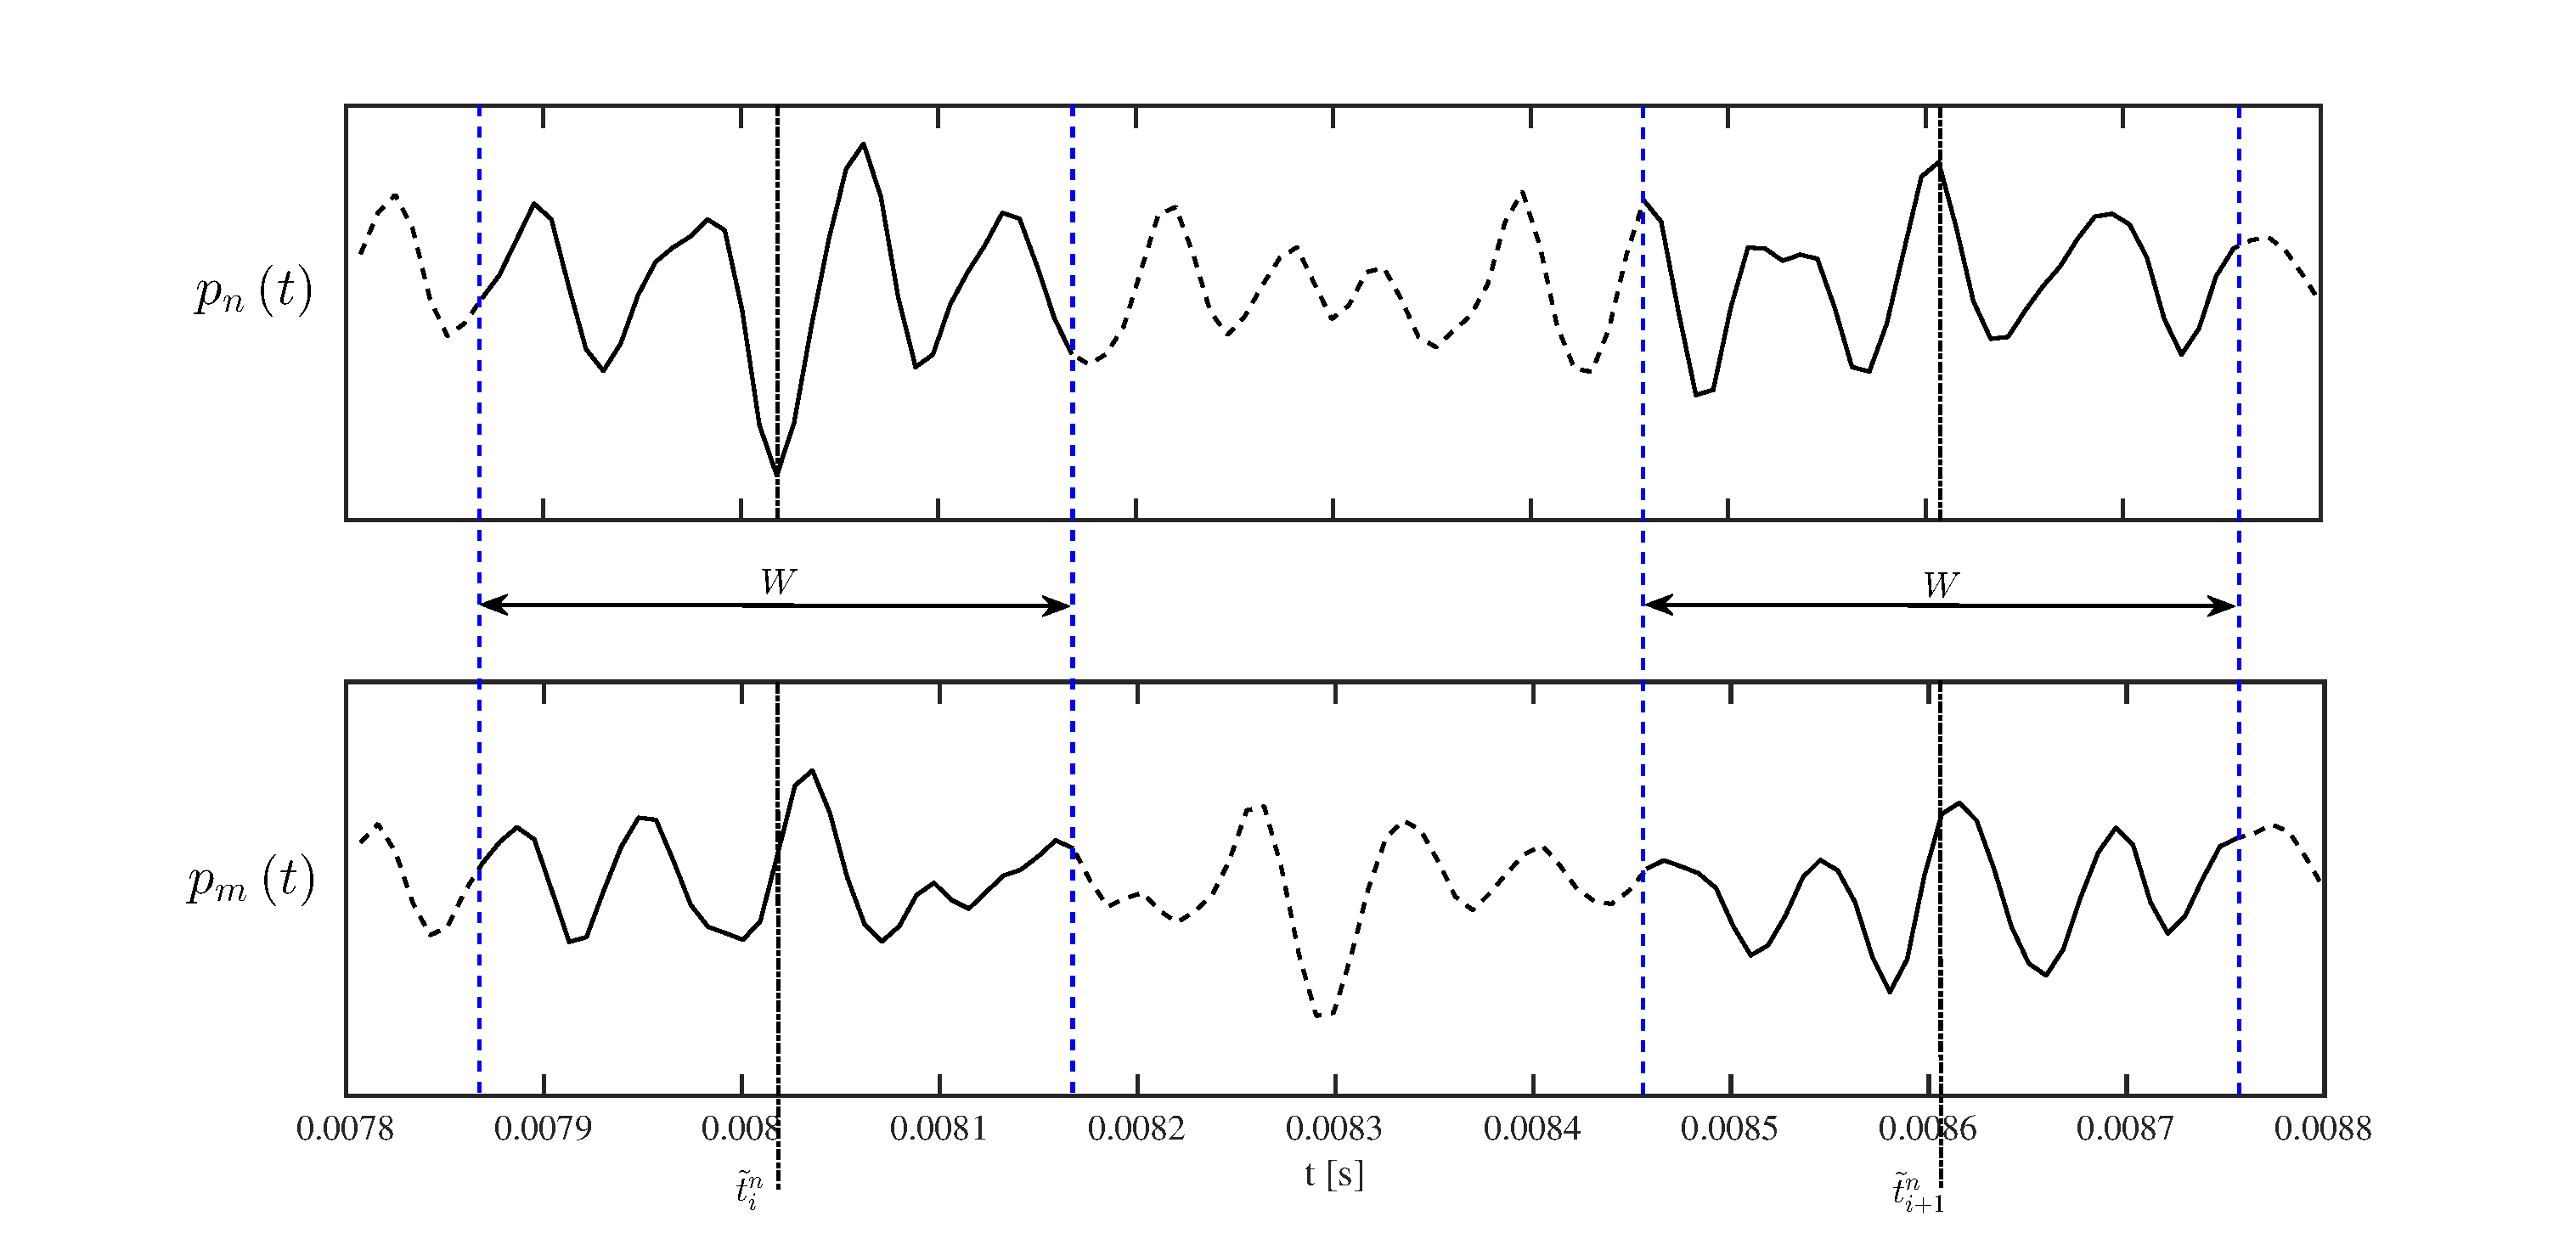
\includegraphics[width=1\textwidth]{Figures/condNcond.eps}
	\caption{\textit{Auto--conditioning of a signal $p_n(t)$ and cross--conditioning of a signal $p_n(t)$}}
	\label{fig:condNcond}
\end{figure}

For sake of brevity, only the results for four different cases, baseline and $S_t = 0.05, 0.25,$ and $0.35$, are presented. The following figure (\fig{fig:autoCondSt0p00}) represents the auto--conditioning of closest microphones array at $r/D = 1.2$ and for the microphones contained between $x/D=1$ and $x/D=14$. Here, only the positive peaks are used to perform the conditional--average. The reason will be explained later with a forced case. The results are non-dimensionalized by the local standard deviation. The first observation is that the energetic event detected using the wavelet--conditioning consists of a positive (or negative) central peak surrounded by two smaller lobs of the opposite sign. The local time--scale of the fluctuation grows as it is convected downstream. It is an expected result and can be reproduced using a simple auto--correlation at each axial position. The interests is to be able to appreciate the variation of the amplitude of the event according to its axial position. Up to $x/D=10$, the amplitude of the event is greater than the local standard deviation by at least twice. Then the fluctuation seems to get weaker and weaker as it is convected further downstream. 

\begin{figure}
	\centering
	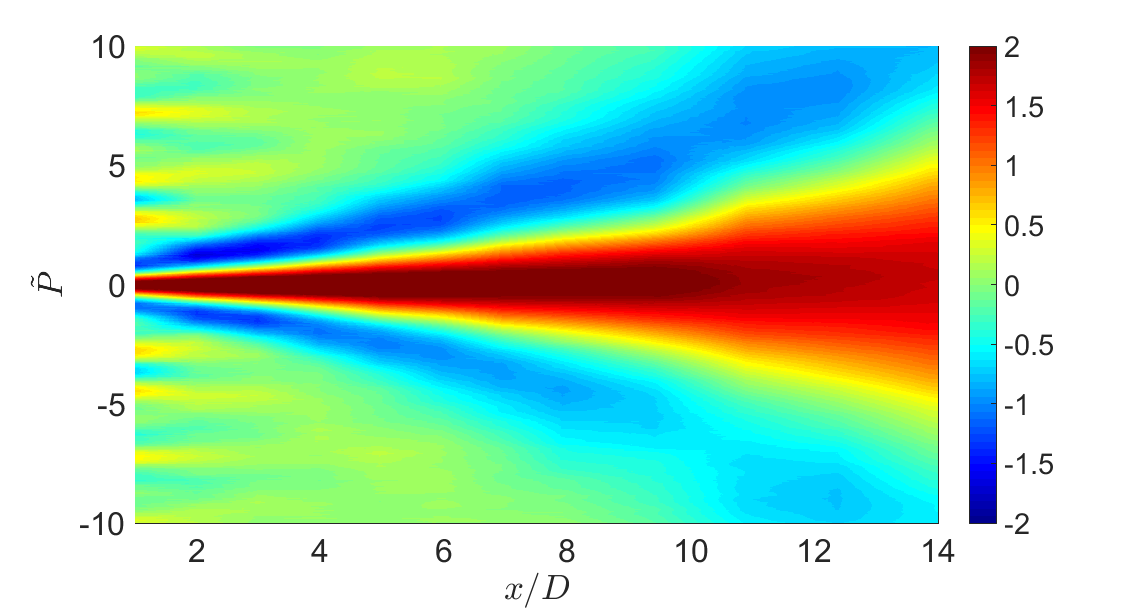
\includegraphics[width=1\textwidth]{Figures/conditioning/autoCondSt0p00.png}
	\caption{\textit{Auto--conditioning of a signal $p_n(t)$ and cross--conditioning of a signal $p_n(t)$}}
	\label{fig:autoCondSt0p00}
\end{figure}

The next figure \fig{fig:autoCondSt0p05} represents the auto--conditioning using the forced case at $S_t = 0.05$. The shape of the energetic event is different with compare to the previous case: it consists of a central peak, here positive, followed by a negative lob. The negative lob is at first of the same amplitude as the central peak and is becoming weaker as the event is convected further downstream. It is interesting to see that downstream, from around $x/D=8$, the energetic event shape of the excited case becomes more similar to the baseline, consisting of a central peak and surrounded by two lobs of the opposite sign. This is the reason of why the conditional--average is done using only the positive (or negative) peaks. The region in which the central peak start to strongly becomes weaker is closer to the nozzle exit, in this case around $x/D = 8$. 

\begin{figure}
	\centering
	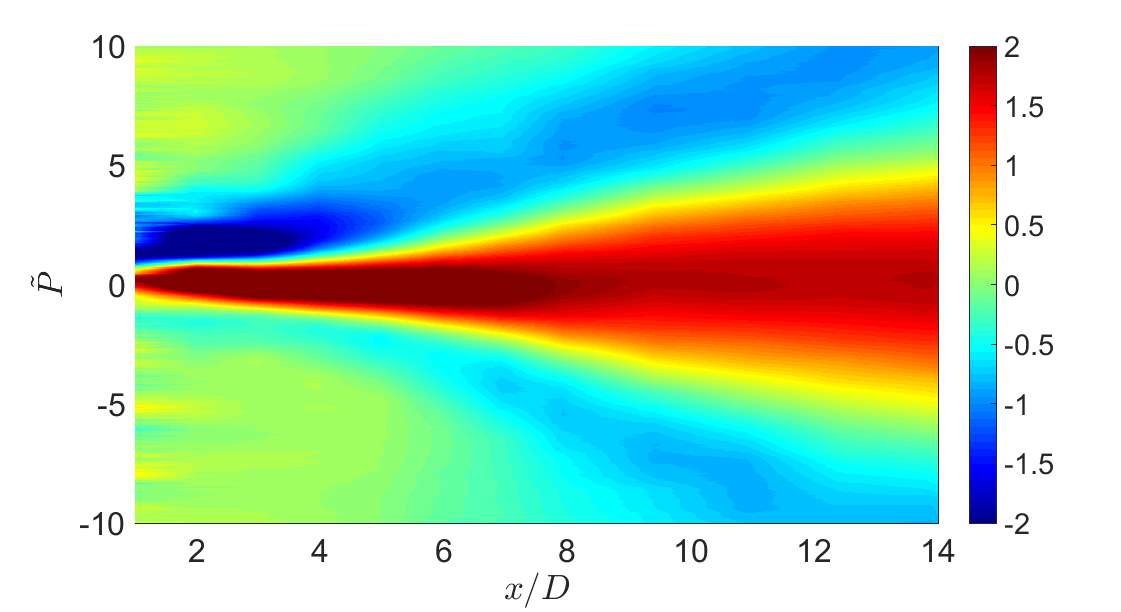
\includegraphics[width=1\textwidth]{Figures/conditioning/autoCondSt0p05.png}
	\caption{\textit{Auto--conditioning of a signal $p_n(t)$ and cross--conditioning of a signal $p_n(t)$}}
	\label{fig:autoCondSt0p05}
\end{figure}

The highest forcing cases are presented next. It can be observed from figures \fig{fig:autoCondSt0p25} and \fig{fig:autoCondSt0p35} that there are many similarities between these two cases. Using the same time scale of the two previous cases, it can be observed multiple energetic events on the same figure. For the case $S_t = 0.25$ case, the energetic event seems to be the same as $S_t = 0.05$. For the highest case it is more difficult to observe it as the time between two successive energetic events is really short and so two successive events are overlapping each other. 

\begin{figure}
	\centering
	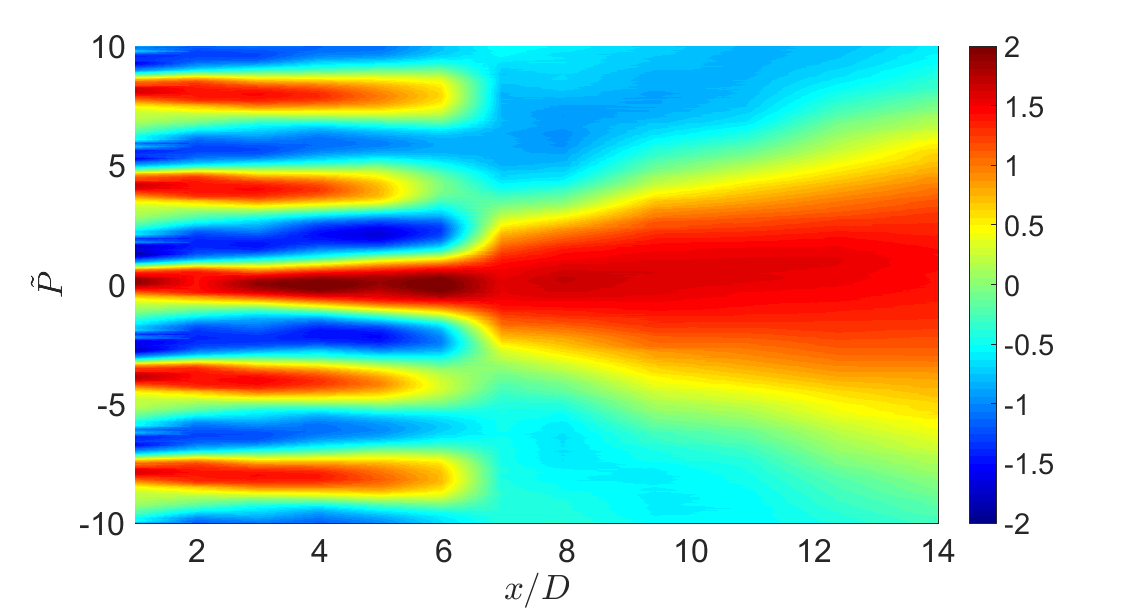
\includegraphics[width=1\textwidth]{Figures/conditioning/autoCondSt0p25.png}
	\caption{\textit{Auto--conditioning of a signal $p_n(t)$ and cross--conditioning of a signal $p_n(t)$}}
	\label{fig:autoCondSt0p25}
\end{figure}

\begin{figure}
	\centering
	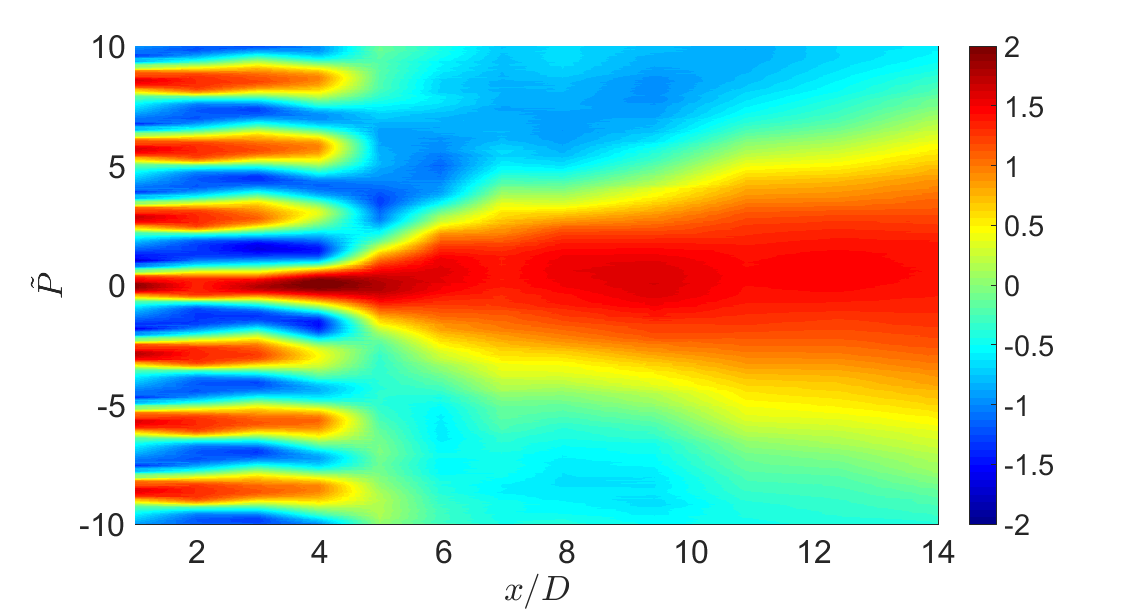
\includegraphics[width=1\textwidth]{Figures/conditioning/autoCondSt0p35.png}
	\caption{\textit{Auto--conditioning of a signal $p_n(t)$ and cross--conditioning of a signal $p_n(t)$}}
	\label{fig:autoCondSt0p35}
\end{figure}
The characteristic energetic--events of the forced cases are not similar in shape to the baseline, a central peak surrounded by two smaller of the opposite sign. It can be noted that the distance from the nozzle on which the excitation takes effect is becoming shorter as the excitation is higher: on figure \fig{fig:autoCondSt0p25} the excitation seems to maintain up to $x/D=6$ while on the following figure, \fig{fig:autoCondSt0p35}, it is up to $x/D=4$, shortened by around $2D$ with compare to the lowest case. 
%%%%%%%%%%%%%%%%%%%%%%%%
All the figure presented in this section are time--structures. It is possible to obtain spatial structures by doing the conditional average in space instead in time. To do so, 

\subsection{Identifying the Acoustic Source Region}
\label{sect:near_field_source_region}
Much of the difficulty in identifying the aeroacoustic source terms revolves around the dissimilar range of scales and fluctuation intensities of the turbulent eddies in the shear layer and the resulting radiated noise. 
Outside the jet shear layer, in the irrotational near-field of the jet, strong hydrodynamic pressure fluctuations associated directly with the passage of coherent structures in the shear layer and their resultant weak acoustic radiation coexist \citep{Arndt1997}. 
Beyond this, in the acoustic far-field, the hydrodynamic signature of the coherent structures is nonexistent owing to their strong exponential decay with radial distance.
Owing to this, identification of pure acoustic waves and their corresponding source events is problematic.
A decomposition of the pressure field into its constitutive hydrodynamic and acoustic components is therefore required. 
By identification and prediction of coherence nulls in the near field, \citet{Coiffet2006} showed that the full irrotational near-field consistent primarily as a linear superposition of its hydrodynamic and acoustic components, which lead subsequent researchers to propose linear filters to extract the individual components from the near-field pressure, with varying degrees of success. 

As discussed by \citet{Tinney2008}, in a transonic jet in which the large-scale structures are convecting subsonically with respect to the ambient speed of sound, a demarcation of the hydrodynamic and acoustic energy fields can be observed with phase velocity.
This is because the hydrodynamic pressure fluctuations will be aligned with the jet axis, and traveling subsonically. 
Acoustic pressure fluctuations will impinge on the linear microphone array at oblique angles, and therefore will appear as having either sonic or supersonic phase velocity, based on the source location. 
Therefore, a demarcaction between the hydrodynamic and acoustic energy components should be readily identifiable about the sonic wavenumber, $k_a = \omega / a_\infty$.
Decomposition of the irrotational near-field pressure is therefore straightforward in Fourier space.

However, there is also a great drawback associated with Fourier analysis: while it analyzes a given signal at a distinct frequency, local information for a given event is spread over all spectral coefficients. 
This is due to the fact that the basis functions used by the Fourier transform oscillate indefinitely. 
For a signal composed of completely random fluctuations this is not an issue, however it has become increasingly clear that the jet noise phenomenon is not a random process \citep{Kearney-Fischer2013}.
Transient events, such as intermittency or the spatial and temporal modulation of a wavepacket, have been shown to be important in the noise generation process. 
It was for this reason that a continuous spatio-temporal wavelet filter, based off of the work of \cite{Antoine2004} and \cite{Kikuchi2010}, was instead used in the current work to decompose the acoustic and hydrodynamic near-fields based on phase-velocity.
It has been shown that by using a temporally/spatially localized fluctuation as a basis, the wavelet transform compresses the information in a turbulent field much more efficiently (and accurately) than the Fourier transform \citep{Farge1992}.
A much more detailed explanation of the spatio-temporal wavelet transform, the justification for its use in decomposing the near-field pressure, and validation of the methodology using the current database can be found in \citet{Crawley2016}. 

By decomposing the irrotational near-field pressure, the relationship between the near- and far-field can be more easily elucidated. 
Two-point correlations were computed using both the full near-field and the acoustic near-field component, between each microphone in the near field and the far-field microphone at $30^\circ$; results can be found in \fig{fig:ch3_full_vs_partial_xcorr}. 
Examination in the spatio-temporal domain shows distinct regions of positive and negative correlation spanning several jet diameters and flow time scales.
The time lag, $\tau$, in the figures have been non-dimensionalized by the ambient speed of sound, $a_\infty$, and $R$, the distance from each near-field microphone to the far-field microphone (note that this results in an ordinate that is scaled separately along the abscissa, due to the dependence of the axial position on $R$).
\begin{figure}
	\centering
		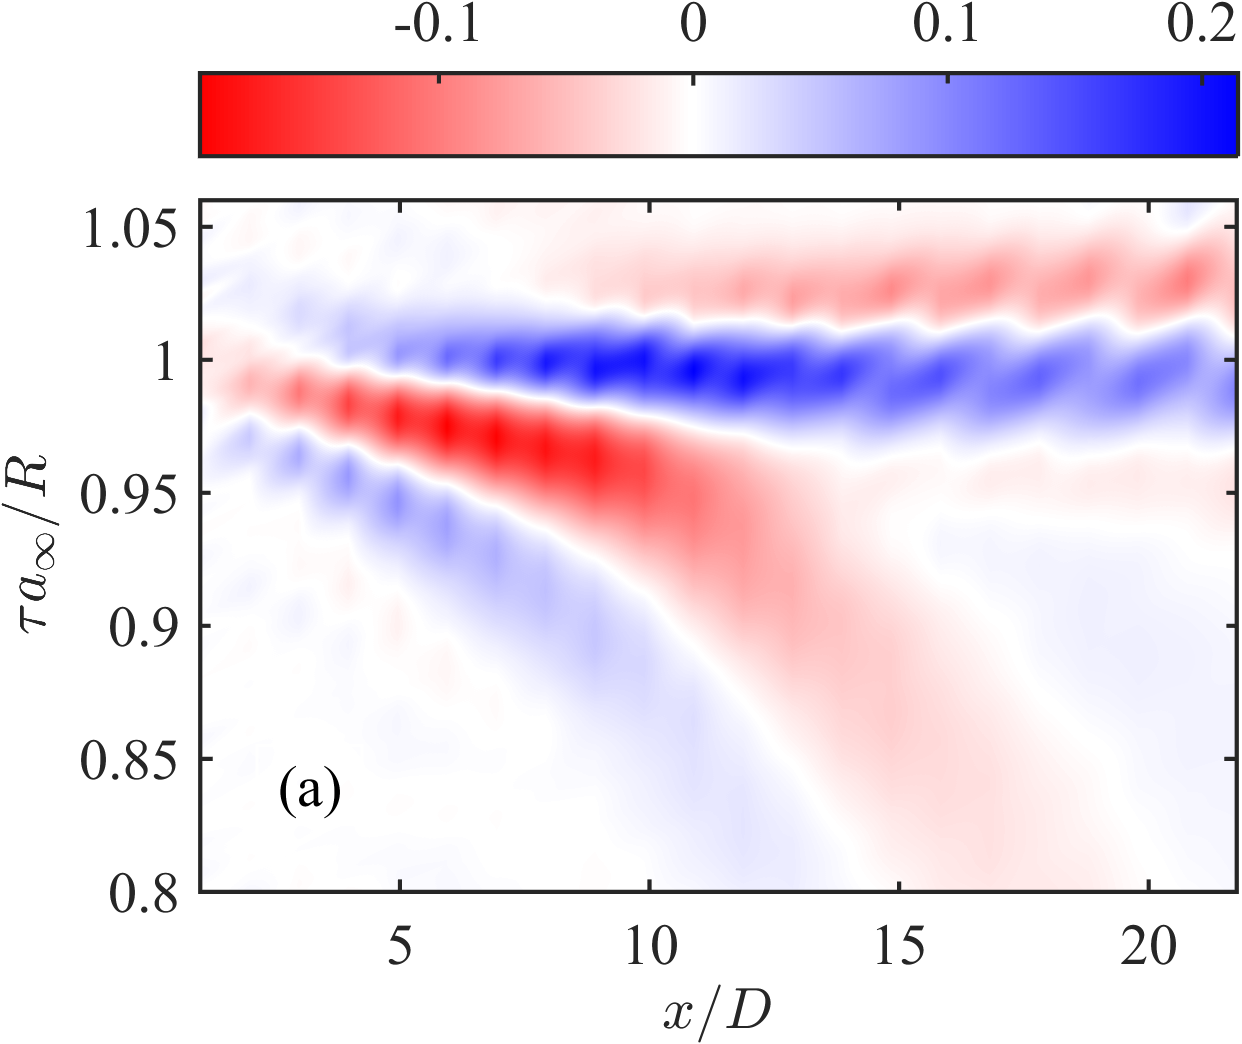
\includegraphics[width=0.475\linewidth]{Figures/sect_nearfield_fullxcorr.png}
		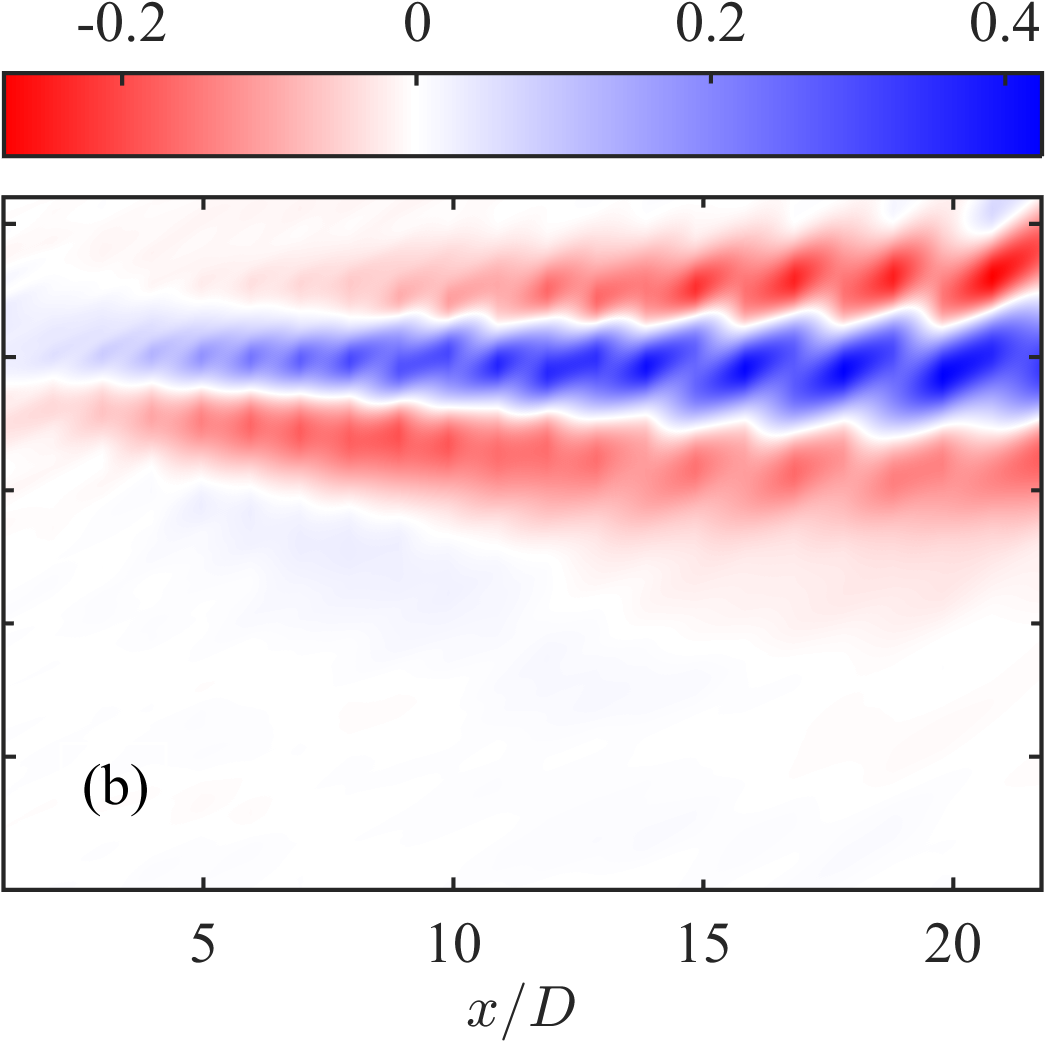
\includegraphics[width=0.401\linewidth]{Figures/sect_nearfield_acousticxcorr.png}
	\caption{Normalized two-point correlations for the natural jet between the near field and the far field at $30^\circ$ for the full near-field pressure (a) and the acoustic component only (b).}
	\label{fig:ch3_full_vs_partial_xcorr}
\end{figure}

Near the jet shear layer (\fig{fig:ch3_full_vs_partial_xcorr}a), four distinct correlation regions can be observed: two positive, two negative; one strong and one weak for each. 
The first correlation regions, the strong-negative and weak-positive, are noticeable beginning at the most upstream microphone and reach their peak values around $5 < x/D < 10$, decaying significantly beyond that.
The slopes of these regions indicate propagation velocities noticeably below the sonic velocity; in the upstream region, they roughly match with the measured convective velocity of the large-scale structures ($U_c \simeq 0.7 U_j$ as measured by two-point correlations between subsequent near-field microphones, see \citet{Crawley2015} for additional details) in the upstream region of the jet, and slowly decelerate downstream.
Similar behavior was observed by \citet{Bogey2007}, who noted that two-point correlations between the flow-field and acoustic near-field in a simulated jet produced strong positive correlation regions which peaked at the end of the potential core and which followed the convection of the large-scale structures.
Conversely, the strong-positive and weak-negative correlation regions exhibit propagation velocities that match well with the ambient speed of sound. 
The distinctly different propagation velocities and of the two pairs of correlation regions indicate that these correspond to different physical phenomena.
The strong-negative and weak-positive correlation regions observed near the jet shear layer are associated with the large-scale structures themselves, rather than acoustic phenomena. 
This relationship becomes even more clear when just the acoustic component of the near-field is considered, rather than the full irrotational near-field. 
Gone entirely now are the correlation regions with subsonic propagation velocities (\fig{fig:ch3_full_vs_partial_xcorr}b), and instead, a single positive correlation region corresponding to sonically-propagating waves exists over the entire domain. 

The correlations of the decomposed near-field can be used to identify the acoustic source region, at least in a rough sense, by comparing the time lag at which the greatest correlation is achieved against expected times-of-arrival for different propagation paths.
A schematic of these propagation paths is provided in \fig{fig:ch3_ToA}.
The first expected time of arrival, $\tau_a$, corresponds to the expected time lag for an acoustic wave traveling directly from the noise source to the near-field microphone and on to the far-field microphone and hence, the noise source region lies along the axis created by the near-field and far-field microphones.
Another expected time-of-arrival can be constructed by assuming the source region is stationary in space; from simple geometric considerations of the distance from the assumed source region to the near-field and far-field microphones, the time lag, $\tau_s$, between the arrival of an acoustic wave at both microphones can be computed.
The stationary source region is of course not known \textit{a priori}, but is set by the author subsequent to the computation of the two-point correlations.

For simplicity, density and convection effects on the acoustic wave as it travels through the jet shear layer have been neglected in this analysis. 
By necessity, it has been assumed that the acoustic radiation in the jet is dominated by $m = 0$ azimuthal Fourier mode (the near-field and far-field microphone arrays are not at the same azimuthal angle with respect to the nozzle). 
This assumption is easily justified in the excited jets, where the actuators have been fired in phase. 
While the near-field pressure and acoustic radiation towards aft polar angles in a natural, high Reynolds number jet is a combination of numerous azimuthal Fourier modes, previous researchers have found these fields to be dominated by the axisymmetric mode \citep{Arndt1997,Hall2006,Koenig2013,Juve1979}.
\begin{figure}
	\centering
	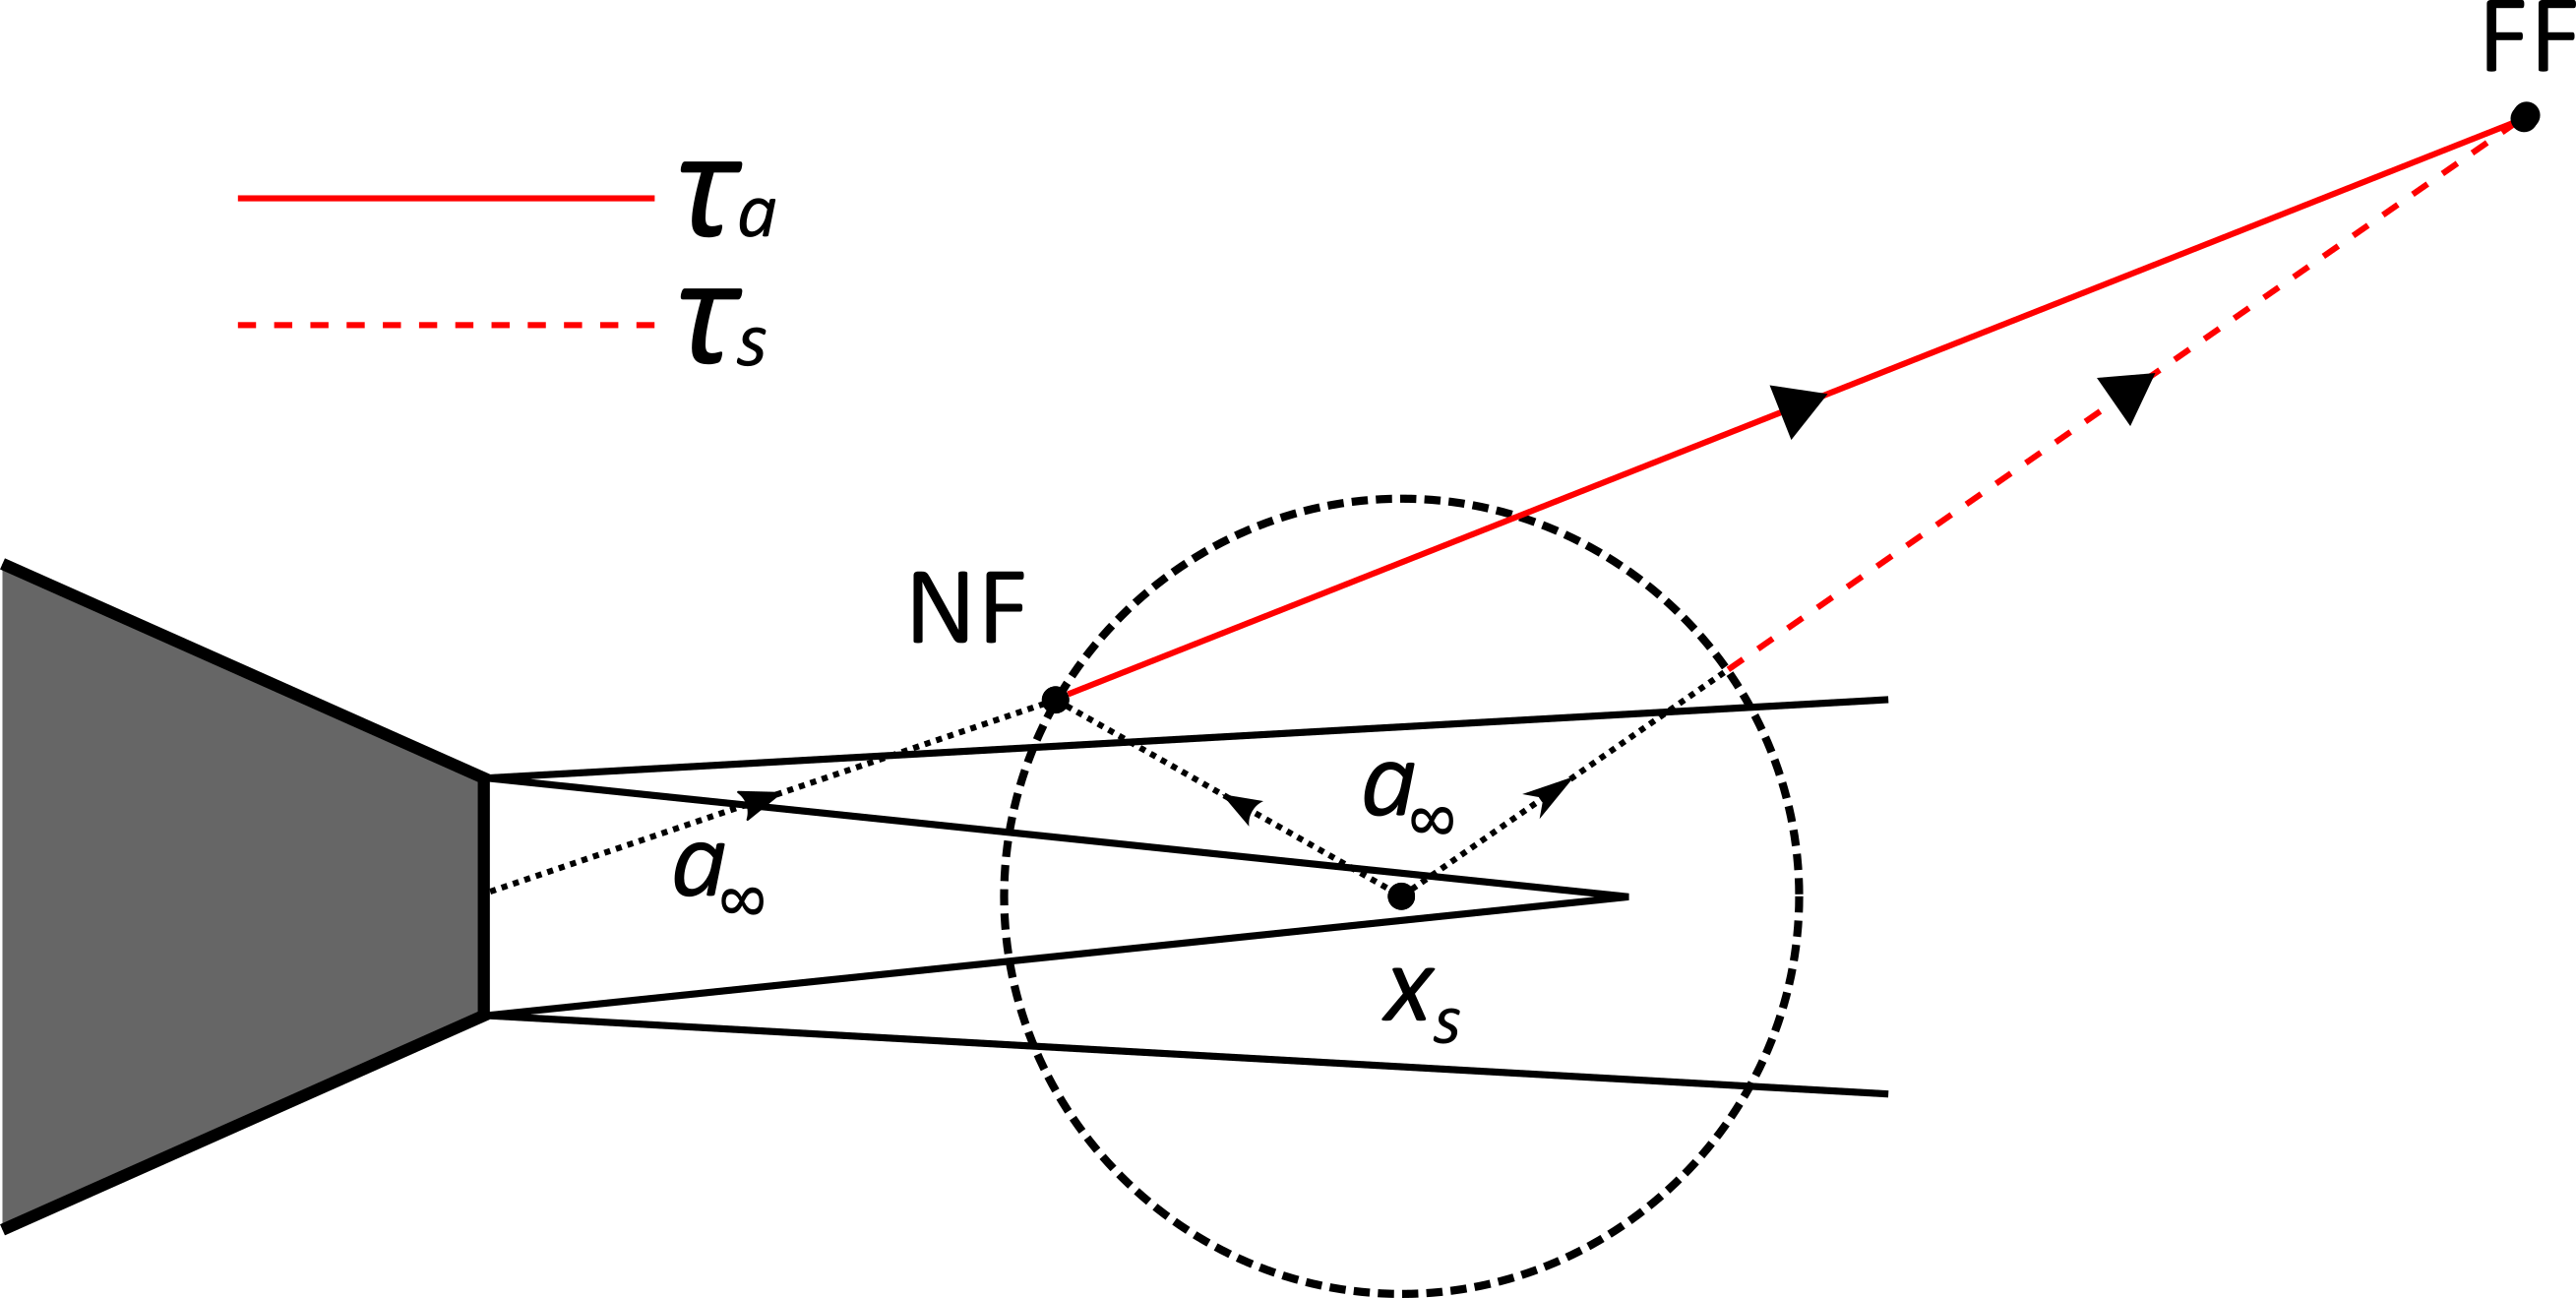
\includegraphics[width=3in]{Figures/ToA_tau.png}
	\caption{Expected times of arrival for on-axis acoustic propagation, $\tau_a$, and off-axis acoustic propagation, $\tau_s$ from a stationary source region centered at $x_s$.}
	\label{fig:ch3_ToA}
\end{figure}

Here, the acoustic source region was assumed to be located at $x_s /D = 4$, which is just upstream of the end of the potential core in the unforced jet. 
(Please note that this analysis is not meant to imply that the source region is located at a specific, fixed point – it is merely a convenient way of understanding the propagation paths.)
Similar behavior is observed between the natural jet and the excited cases in \fig{fig:ch3_xcorrOA}; note that due to numerical discrepancies at the domain boundaries (see \citet{Torrence1998} for a discussion of the `cone of influence' of wavelet coefficients and the effect thereof), the correlation values have been truncated at the most upstream and downstream microphones.
For the impulsively-excited jet, nearly identical correlation regions are observed between the excited and natural jet; in the periodically-excited jet continuous oscillations occur throughout time due to the similarity of continuously-generated large-scale structures and resultant acoustic radiation.
In the upstream region of the jet, the peaks of the positive correlation region match $\tau_a$ nearly exactly. 
In the downstream region, $\tau_a$ begins to increasingly over-predict the time lag for the maximum correlation. 
On the other hand, $\tau_s$ tracks the time lags for the peak correlation consistently over the downstream region, but not the upstream region. 
The results found here appear to indicate that the dominant acoustic radiation reaching the far-field aft angles is being generated over an extended region of the jet mixing layer, roughly $x/D \leq 4$, which is just upstream of the time-averaged end of the potential core in the natural jet.
This is not too dissimilar from the findings of other researchers, who have suggested that the acoustic source region lies just \textit{downstream} of the end of the potential core \citep{Hileman2005}.
It should be clarified here though, that the interpretation of these results is not meant to suggest that only trivial levels of noise are generated outside of this apparent noise source region, just that the dominant radiation is produced in this region in a time-averaged sense.
\begin{figure}
	\centering
	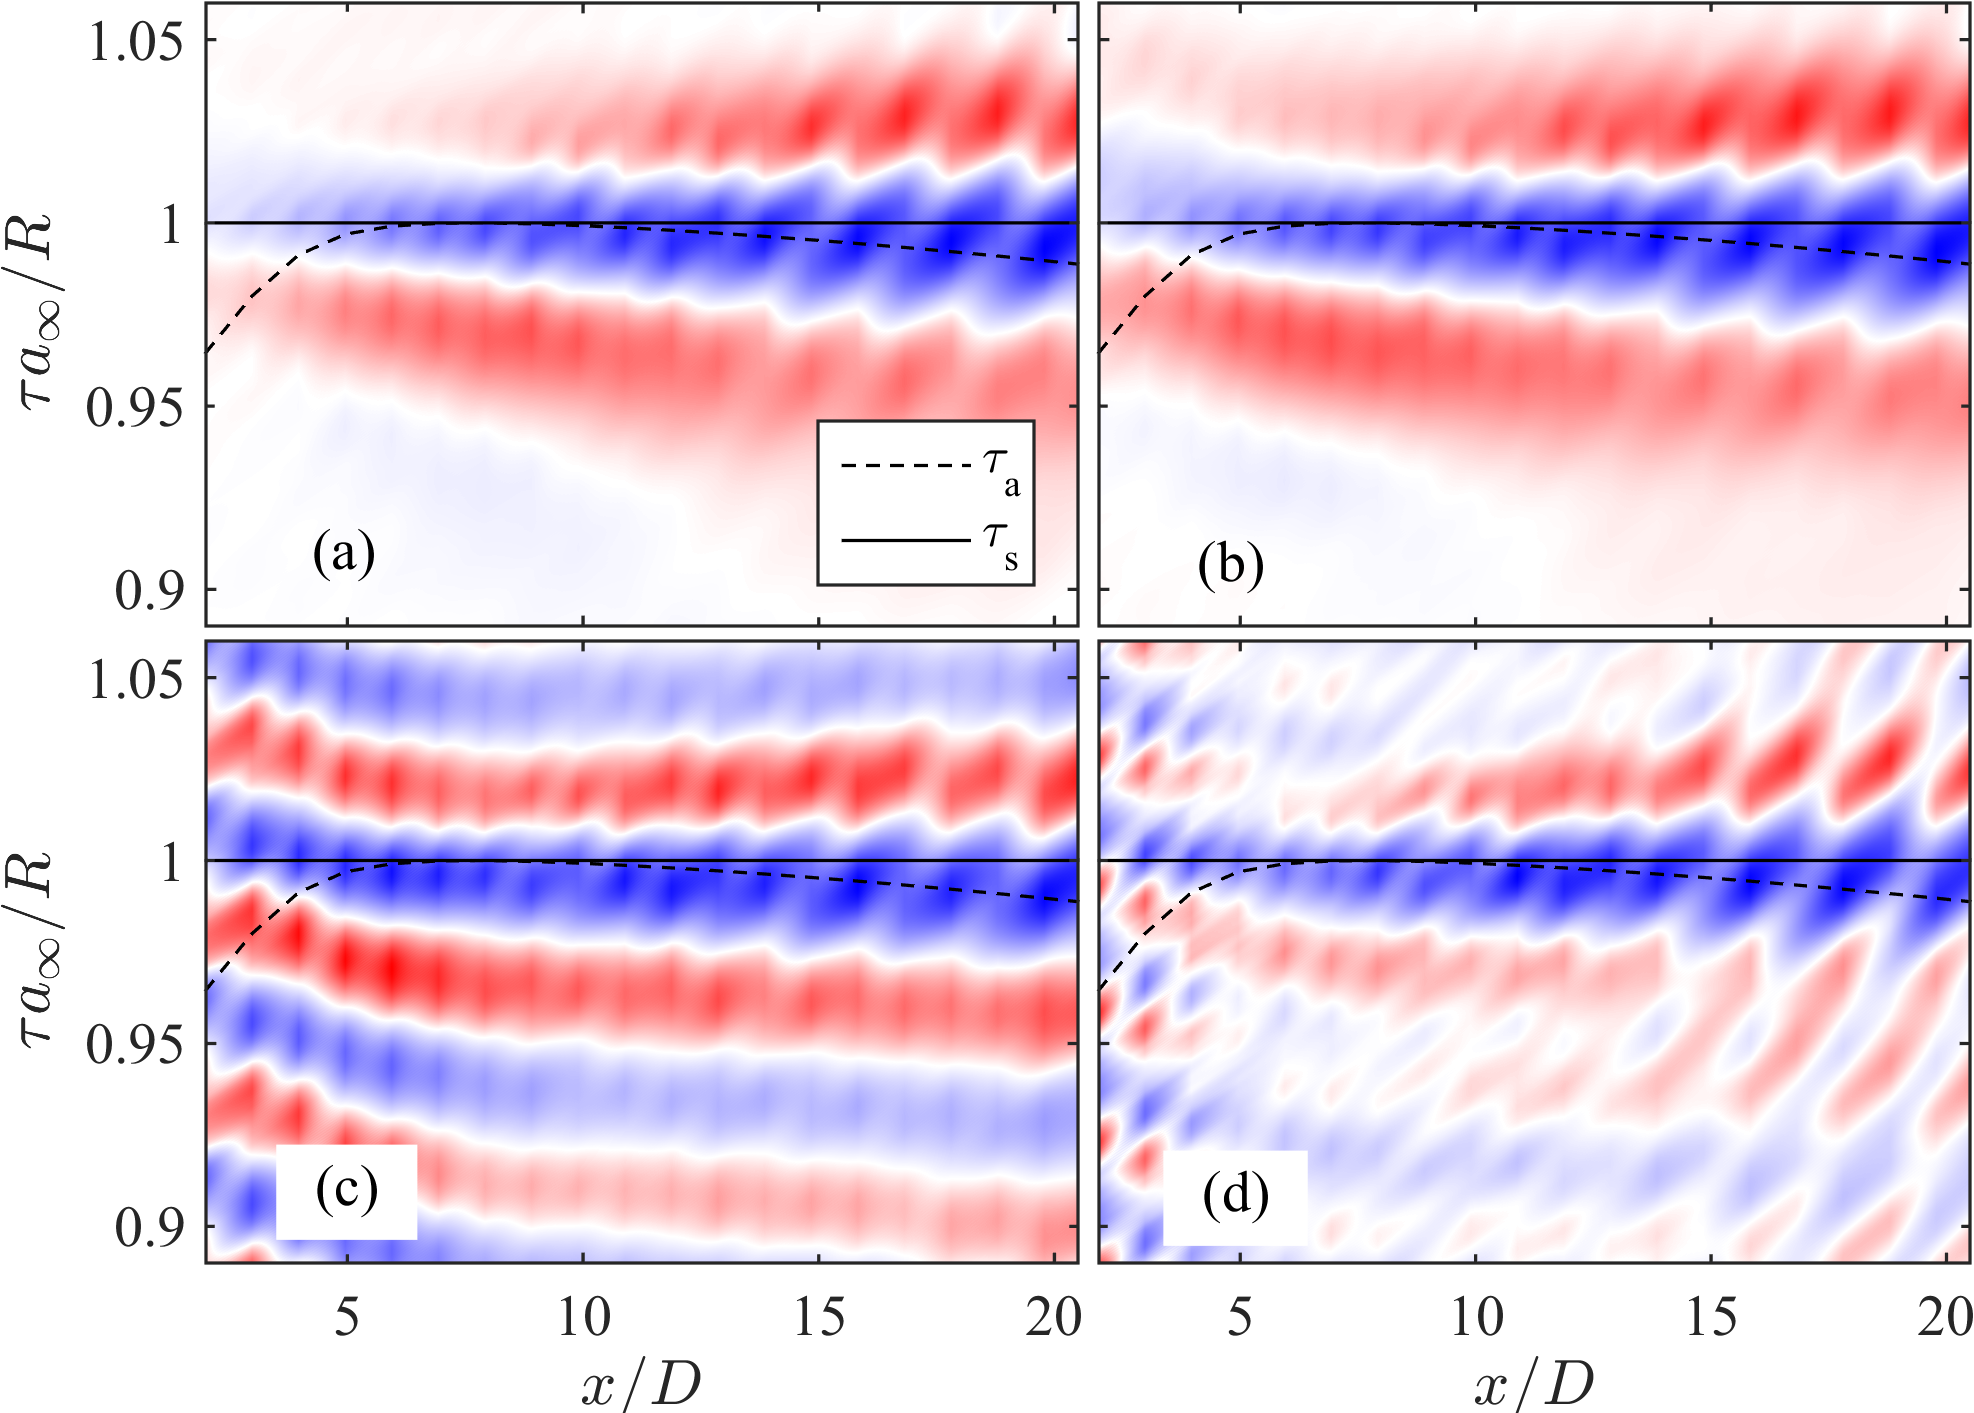
\includegraphics[width=\linewidth]{Figures/sect_nearfield_ffxcorr.png}
	\caption{Normalized two-point correlations between the acoustic component of the near field and the far field at $30^\circ$ for microphone array position starting at $x/D = 1, r/D = 1.2$ for the natural jet (a), $St_{DF} = 0.05$ (b), $St_{DF} = 0.25$ (c) and $St_{DF} = 0.35$ (d).}
	\label{fig:ch3_xcorrOA}
\end{figure}

However, these results should not be interpreted as indicating that the source mechanisms are necessarily consistent for all excitation frequencies. 
For the lower-frequency periodic excitation ($St_{DF} \leq 0.25$), the consistency in the far-field response (\fig{fig:ch3_farfield_linear}) coupled with the consistency in the apparent source region is suggestive of a consistent dominant source mechanism.
In contrast, the inconsistency in the far-field response for the higher-frequency periodic excitation ($St_{DF} \geq 0.35$, \fig{fig:ch3_farfield_nonlinear}) is suggestive of a change in the dominant source mechanism, just one that is associated with the vortex dynamics in the jet shear layer upstream of the end of the potential core.
It should also be noted that the peak correlation values between the acoustic near-field and the far-field are significantly lower (though certainly non-negligible) in the periodic excitation cases, suggesting a decaying coherence in the source mechanisms at these frequencies.
From the current results alone, the significance of this estimated source region is not entirely clear.
In \sect{sect:velocity} the time-resolved velocity field will be explored in detail to better elucidate the structure dynamics, with a particular focus on the region just upstream of the end of the potential core.

The authors would like to make a special note here, concerning the discrepancy between the results presented in \fig{fig:ch3_xcorrOA} and those presented previously in \citet{Crawley2015}.
In that paper, the more simple Fourier filter was used to decompose the irrotational near-field; processing artifacts were noted and a parametric study was attempted to minimize their impact.
In the resulting two-point correlations of the decomposed acoustic field, a shift in the apparent source region was noted to coincide with the shift of the peak pressure fluctuations measured just outside the shear layer (higher frequency excitation cases saturating further upstream near the nozzle exit).
Because this behavior was observed across the entire range of filter parameters used, it was assumed to be representative of the true physical behavior and not a numerical artifact.
Of course, this assumption precludes the possibility that \textit{the entire parameter space produced similar numerical artifacts}. 
As discussed more thoroughly in \citet{Crawley2016}, the Fourier filter has a tendency to allow energy leakage from the hydrodynamic field into the acoustic, particularly at low frequencies. 
Since it has already been observed that the hydrodynamic signature of the large-scale structures can linearly correlate to the acoustic emission, a potential consequence of this leakage is correlation regions which instead point to the region of high hydrodynamic energy - i.e. the saturation point of the near-field pressure fluctuations.
The analysis found of \citet{Crawley2016} demonstrated that wavelet filter is far more robust to energy leakage and numerical artifacts, and as such the authors is inclined to lend more credence to the results presented herein. 